
% !TeX spellcheck = de_DE
\documentclass{article}

\usepackage[ngerman]{babel}
\usepackage{graphicx}
\usepackage{indentfirst}
\usepackage{hyperref}
\usepackage{geometry}
\usepackage{changepage}
\usepackage{booktabs}
\usepackage{float}
\usepackage{tabulary}
\usepackage{multirow}

\graphicspath{ {./images/} }
\setlength\parindent{0pt}

\makeatletter
\newcommand{\sectionauthor}[1]{
	{\parindent 0em \large \scshape Autor: #1 \par \nobreak \vspace*{1em}}
	\@afterheading
}
\newcommand{\specification}[3]{
	{\parindent 0.5em \hangindent 3em \hypertarget{spec:#1:#2}{\textbf{/#1#2/}} #3 \par \nobreak \vspace*{0.5em}}
}
\makeatother

\begin{document}

%--Einleitung--------------------------------------------------------------------------------------------------------------------------------------------------------------------------
\section{Einleitung}
\sectionauthor{Jonas Picker}
Hier wird der Entwurf des Bibliotheksmanagementsystems BiBi beschrieben. Das Dokument bezieht sich auf das Lastenheft von Christian Bachmaier und Armin Größlinger und stellt eine technische Vertiefung unseres Pflichtenhefts dar, welches im Folgenden wiederholt referenziert wird.

%--Systemarchitektur---------------------------------------------------------------------------------------------------------------------------------------------------------------
\section{Systemarchitektur}
\sectionauthor{Ivan Charviakou}



\subsection{Einführung}

Die vorgestellte Bibliotheksanwendung wird in Java mittels einer MVC-Architektur unter Verwendung eines 2-Schichten Modells realisiert. Dabei wird JSF als grundlegendes Web-Framework verwendet. Der Vorteil dieser Modellierung ist die Einfachheit der Implementierung und die Modularität der Datenschicht. Aufgrund der wenig umfangreichen Businesslogik bietet aber eine separate Schicht im Gegensatz zum 2-Schichten Modell bei deutlichem Mehraufwand kaum zusätzliche Modularität. \vspace{0.5em}

Genauer – Das Model besteht aus den folgenden Schichten:
\begin{itemize}
	\item \textbf{Logikschicht:} Die Aufgabe dieser Schicht ist es, die Benutzerinteraktion, die Navigation, und die hierzu erforderliche Funktionalitäten zu kapseln. 
	\item \textbf{Datenschicht:} Da manche Funktionalitäten aus der Logik eine Datenpersistenz voraussetzen, befasst sich diese Schicht mit dem Speichern und Laden von Daten aus einem oder mehreren Quellen.
\end{itemize}



\subsection{Architekturdiagramm}

Das folgende Diagramm stellt die MVC-Architektur mit den Beziehungen zwischen den einzelnen Komponenten anhand der gegebenen Applikation dar. Dabei folgt die Komponentenaufteilung grob der Paketstruktur der Applikation. Zudem entsprechen die Farben, die die Komponente im Diagramm besitzen, den Farben im nachfolgenden Klassendiagramm.

\begin{figure}[H]
	\centering
	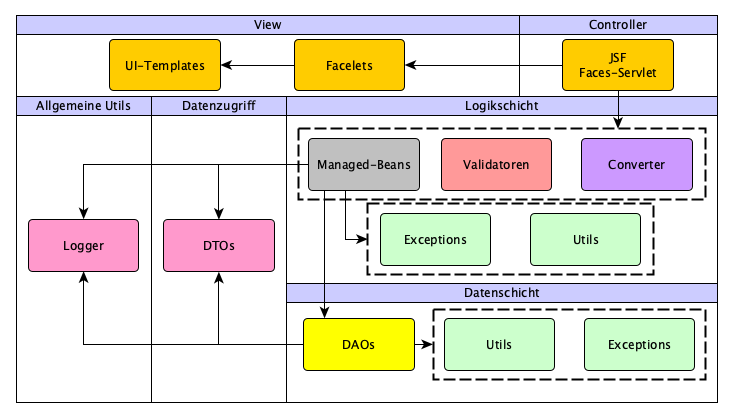
\includegraphics[width = 30em]{Modeldiagramm}
\end{figure}



\subsection{Paketstruktur}

Die verwendeten Java-Paketen werden im Folgenden aufgelistet und beschrieben:
\begin{itemize}
	\item \textbf{dedede.model.logic:} Dieses Paket bildet die gesamte Funktionalität der Logikschicht ab.
		\begin{itemize}
			\item \textbf{dedede.model.logic.managedbeans:} Dieses Paket enthält alle von der JSF-Applikation verwendeten Managed-Beans. 
				Das sind unter anderem Backing-Beans, die von den Facelets referenziert werden, und jegliche Scoped-Beans, die diesen Backing-Beans zusätzliche Funktionalität bieten.
			\item \textbf{dedede.model.logic.validators:} Dieses Paket enthält alle von der JSF-Applikation für die Überprüfung der Benutzereingabe verwendeten Validatoren.
			\item \textbf{dedede.model.logic.converters:} Dieses Paket enthält alle von der JSF-Applikation verwendeten Converters.
			\item \textbf{dedede.model.logic.exceptions:} Dieses Paket definiert alle applikations-spezifische Exceptions, die von den Klassen aus der Logikschicht geworfen werden. 
				Insbesondere sind das checked und unchecked Exceptions, die nur in der Logikschicht eine kontextuelle Bedeutung tragen.
			\item \textbf{dedede.model.logic.util:} Dieses Paket kapselt alle Funktionalitäten, von der die Funktionsweise der Logikschicht abhängt, aber auch über die direkte Benutzerinteraktion hinausgehen. 
				Das sind unter andrem die E-Mail-Versendungsfunktionalität und die SystemEventListener-Implementierung, die für den Logikschicht-gesteuerten Systemstart und -stopp zuständig ist.
		\end{itemize}
	\item \textbf{dedede.model.dataaccess:} Dieses Paket bildet die gesamte Funktionalität der Datenschicht ab.
		\begin{itemize}
			\item \textbf{dedede.model.dataaccess.daos:} Dieses Paket enthält alle von der Applikation verwendeten Datenzugriffsobjekten (DAOs).
			\item \textbf{dedede.model.dataaccess.exceptions:} Dieses Paket definiert alle applikations-spezifische Exceptions, die von den Klassen aus der Datenschicht geworfen werden. 
				Insbesondere sind das checked und unchecked Exceptions, die nur in der Datenschicht eine kontextuelle Bedeutung tragen.
			\item \textbf{dedede.model.dataaccess.util:} Dieses Paket kapselt alle Funktionalitäten, von der die Funktionsweise der Datenschicht abhängt. 
				Dazu zählen unter anderem das Connection-Pool, das für die Datenbankverbindung notwendig ist, und der Wartungsthread, der die Integrität und Gültigkeit der persistierten Daten überwacht.
		\end{itemize}
	\item \textbf{dedede.model.data:} Dieses Paket stellt dem Applikationsmodell schichtenübergreifende Datenkonstruktionen bereit.
		\begin{itemize}
			\item \textbf{dedede.model.data.dtos:} Dieses Paket enthält alle von der Applikation verwendeten Datentransferobjekten (DTOs).
		\end{itemize}
	\item \textbf{dedede.model.util:} In diesem Paket sind schichtenübergreifende Funktionalitäten und Einstellungen zu finden.
		\begin{itemize}
			\item \textbf{dedede.model.util.logger:} Dieses Paket beinhaltet eine Implementierung eines Loggers und alle hierzu erforderlichen Einstellungen. Dabei ist dieser Logger aus allen Schichten und Klassen zugreifbar.
		\end{itemize}
\end{itemize}


\subsection{Design-Patterns}

\paragraph{Dependency-Injection:} 
In JSF sorgt dieses Pattern dafür, dass eine Managed-Bean-Instanz einer Klasse automatisch bei der Instanziierung zur Verfügung gestellt wird. Dies unterscheidet sich von dem einfachen Anliegen eines Objekts dadurch, dass ein Managed-Bean mit einem größeren, Request-übergreifenden Scope wiederverwendet werden kann. In der gegebenen Anwendung wird dieses Pattern verwendet, um mit Hilfe von Scoped-Beans unter anderem den Applikations- und Session-Zustand zu modellieren. Als Beispiel wird in dem Session-Bean die Rolle eines Nutzers gespeichert, die bei der Nutzeranmeldung gesetzt wird. Durch Dependency-Injection bekommt das Backing-Bean der Medienansicht Zugriff auf diese Rolle, um Rollen-spezifische Funktionalitäten des Facelets anzuzeigen.

\paragraph{Factory-Pattern:} 
Dieses Pattern erlaubt es, Objekte unabhängig von einer bestimmten Implementierung oder Einstellung zu erzeugen. Somit kann eine Implementierung dynamisch gewählt und leichter angepasst werden. 
Um einen globalen Exception-Handler in JSF zu definieren, muss man als Beispiel zuerst den vorgegebenen Exception-Handler-Factory erweitern und diesen in den JSF-Konfigurationen registrieren. 
Dieses Konstrukt erlaubt es, eigene Fehlerbehandlungsprozeduren als Wrapper-Klassen zu definieren, aus denen bei der Konstruktion eines Exception-Handlers ausgewählt wird. 
Die einzige Funktionalität, die der globale Exception-Handler in der gegebenen Anwendung umsetzt, ist die Weiterleitung des Nutzers nur auf eine Fehlerseite. Trotzdem lässt sich mithilfe dieses Patterns weitere Funktionalitäten definieren. 

\paragraph{Singleton-Pattern:} 
Das Singleton-Pattern sorgt dafür, dass ein Objekt im Lebenszyklus der Applikation nur einmal instanziiert wird. Ein wichtiger Vorteil eines Singletons ist die einfache Koordination von bestimmten Operationen. 
In der gegebenen Applikation ist das Connection-Pool als Singleton realisiert. Dadurch wird unter anderem ein koordiniertes Herunterfahren aller Connections im System ermöglicht.

\paragraph{Object-Queuing:} 
Dieses Pattern dient dazu, die Erzeugung von bestimmten Objekten zu beschränken und diese durch Vergabe und Rückgabe wiederverwendbar zu machen. Dies wird häufig in Fällen eingesetzt, in denen die Erzeugung von den Objekten als aufwendig gilt. 
Durch Anwendung dieses Patterns werden die Connections aus dem Connection-Pool in ihrer Anzahl beschränkt, anderen Komponenten zur Verfügung gestellt, und anschließend an den Pool zurückgegeben.

\paragraph{Converter:} 
Ein JSF-Converter hat die Aufgabe, für Objekte eine String-Darstellung zu berechnen, und für eine String-Darstellung ein Objekt. Dies wird in JSF verwendet, um Objekte in der View besser darstellbar oder auswählbar zu machen. 
Beispielsweise sind für sämtliche Auswahllisten, die intern als Enum-Typen kodiert werden, Converter nötig. So werden unter anderem Nutzerrollen und Attributtypen kodiert.

\paragraph{Data Transfer Objects:} 
Dieses Konstrukt kapselt zusammenhängende Daten zu einer oder mehreren Entitäten mit Hilfe von Gettern und Settern. Dabei enthält eine DTO keine Logik und wird als POJO implementiert. 
Zudem werden DTO-Instanzen durch alle Modelschichten durchgereicht und erfüllen in jeder Schicht einen eigenen Zweck. 
In der Datenschicht werden DTOs an DAOs übergeben und verwendet, um persistente Entity-Instanzen im Datenbestand zu aktualisieren, erstellen, oder löschen. DAOs dürfen auch DTOs erzeugen und befüllen. 
In der Logikschicht werden DTOs zum einen aus der Datenschicht geholt, um persistierte Daten in der View anzuzeigen. Zum anderen werden sie in der Logikschicht durch Post-Construct-Methoden erzeugt, um von der View befüllt zu werden.

\paragraph{Data Access Objects:} 
Ein DAO wird verwendet, um Daten zu einer oder mehreren Entitäten mit Hilfe eines DTOs aus dem persistenten Datenbestand zu laden, löschen, aktualisieren, oder einzufügen. 
Dabei sind komplexere Methodenformulierungen möglich und die verwendete Art von Datenpersistenz bleibt für die Logikschicht transparent. 
Die DAOs in der gegebenen Anwendung unterstützen Transaktionsmanagement dadurch, dass öffentliche DAO-Steuermethoden package-private Methoden von anderen DAOs aufrufen dürfen. 
Da die Implementierung der DAOs auf SQL ausgerichtet ist, werden Connection-Objekte durch diese package-private Methoden übergeben. Folglich sind die DAOs als statische Klassen realisiert.

\paragraph{Observer-Pattern:} 
Dieses Pattern trennt die Rolle eines Observers und die eines Subjekts. Hierbei muss ein Observer dem Subjekt zugewiesen werden, um über Änderungen benachrichtigt zu werden. 
Dadurch muss im Subjekt nicht fest-kodiert werden, wie viele Observer referenziert werden und welchen Typ sie besitzen. 
In JSF liegt dieses Pattern einer Implementierung von einem Event- und Phasen-Listener zugrunde. Diese Listener werden nämlich als Observers verwendet, die auf bestimmte Events reagieren.



\subsection{Fehlerbehandlung}

\paragraph{Validatoren:}
Das in JSF eingebaute Validatoren-Konstrukt dient als erster Schutz gegen fehlerhafte Nutzereingaben. 
In einem Validator wird eine Eingabe aus der View auf Korrektheit geprüft und im Fehlerfall eine Validator-Exception geworfen, die in der View als Folge eine Fehlermeldung erzeugt. 
Als Beispiel von einem Validator aus der gegebenen Applikation dient der E-Mail-Validator. Bevor das System bei einer Registrierung eine E-Mail akzeptiert, wird nämlich überprüft, ob sie zu einem regulären Ausdruck passt. 

\paragraph{Phasen-Listener:} 
Um unberechtigten Zugriff auf View-Ressourcen und Funktionalitäten zu vermeiden, werden mit Hilfe eines Phasen-Listeners die Nutzerberechtigungen geprüft. 
Hierbei wird das Interface ‘PhaseListener‘ von JSF vorgegeben, deren Implementierungen lassen sich in der JSF-Konfiguration registrieren. 
Falls die Nutzerberechtigungen für den angeforderten Zugriff nicht ausreichend sind, wird der Nutzer auf eine Fehlerseite weitergeleitet. 
Der gleiche Mechanismus wird auch dazu verwendet, Tokens für eine Passwortrücksetzung oder E-Mail-Verifizierung zu registrieren oder entfernen. 

\paragraph{Logging:} 
Ein wichtiger Aspekt der Fehlererkennung in der gegebenen Applikation ist das Logging-Framework. Durch einen Logger ist es möglich, den Ablauf der Anwendung und dabei entstehende Ereignisse in einer Log-Datei zu dokumentieren. 
Der in der Applikation verwendete Logger definiert die Levels ‚SEVERE‘, ‚DETAILED‘ und ‚DEVELOPMENT‘ für Log-Einträge. 
Da sowohl die Logik- als auch die Datenschicht den gleichen Logger verwendet, wird er in der gegebenen Applikation als schichtenübergreifendes Singleton implementiert.

\paragraph{Exception-Handling:} 
Für jede Modellschicht werden eigene Checked-Exceptions definiert und verwendet. Die Behandlung oder ggf. das Weiterwerfen von diesen Exceptions geschieht in ‚try-catch‘-Blocken im aufrufenden Code. 
Checked-Exceptions, die aus einer unteren Schicht stammen, können ebenfalls in ‚try-catch‘-Blocken in der oberen Schicht gefangen werden. 
Um aber die Unabhängigkeit der Schichten zu unterstützen, wird stattdessen eine andere, schichten-spezifische Exception erzeugt und weitergeworfen. 
Für die Behandlung von sämtlichen nicht-gefangenen Exceptions wird in der Applikation ein eigener globaler Exception-Handler vorgesehen, der den Nutzer auf eine Fehlerseite weiterleitet und die entsprechenden Details zu dieser Exception anzeigt. 
Das sind unter anderem der Name, die Nachricht, und der Stack-Trace. 



\subsection{Systemvorgänge}

\paragraph{Systemstart und Shutdown:}
Obwohl jede Modelschicht hierzu ihre eigenen Klassen und Prozeduren definiert, wird sowohl ein Systemstart als auch ein Shutdown durch die Logikschicht angestoßen. 
Dies erfolgt durch die Implementierung und Registrierung des ‚SystemEventListeners‘-Interfaces, die aus der Logikschicht die entsprechenden statischen Methoden in der Logikschicht aufruft.

\paragraph{Unerwartetes Shutdown:}
Die Ausführung von Shutdownfunktionen beim unerwarteten Beenden der JVM, wie das Schließen von Datenbankverbindungen und Connection-Objekte, wird mit Hilfe einer Shutdown-Hooks realisiert. 



%--Klassendiagramm---------------------------------------------------------------------------------------------------------------------------------------------------------------

\section{Klassendiagramm}
\sectionauthor{Mohamad Najjar}

%   \begin{landscape}
    \begin{figure}[H]
        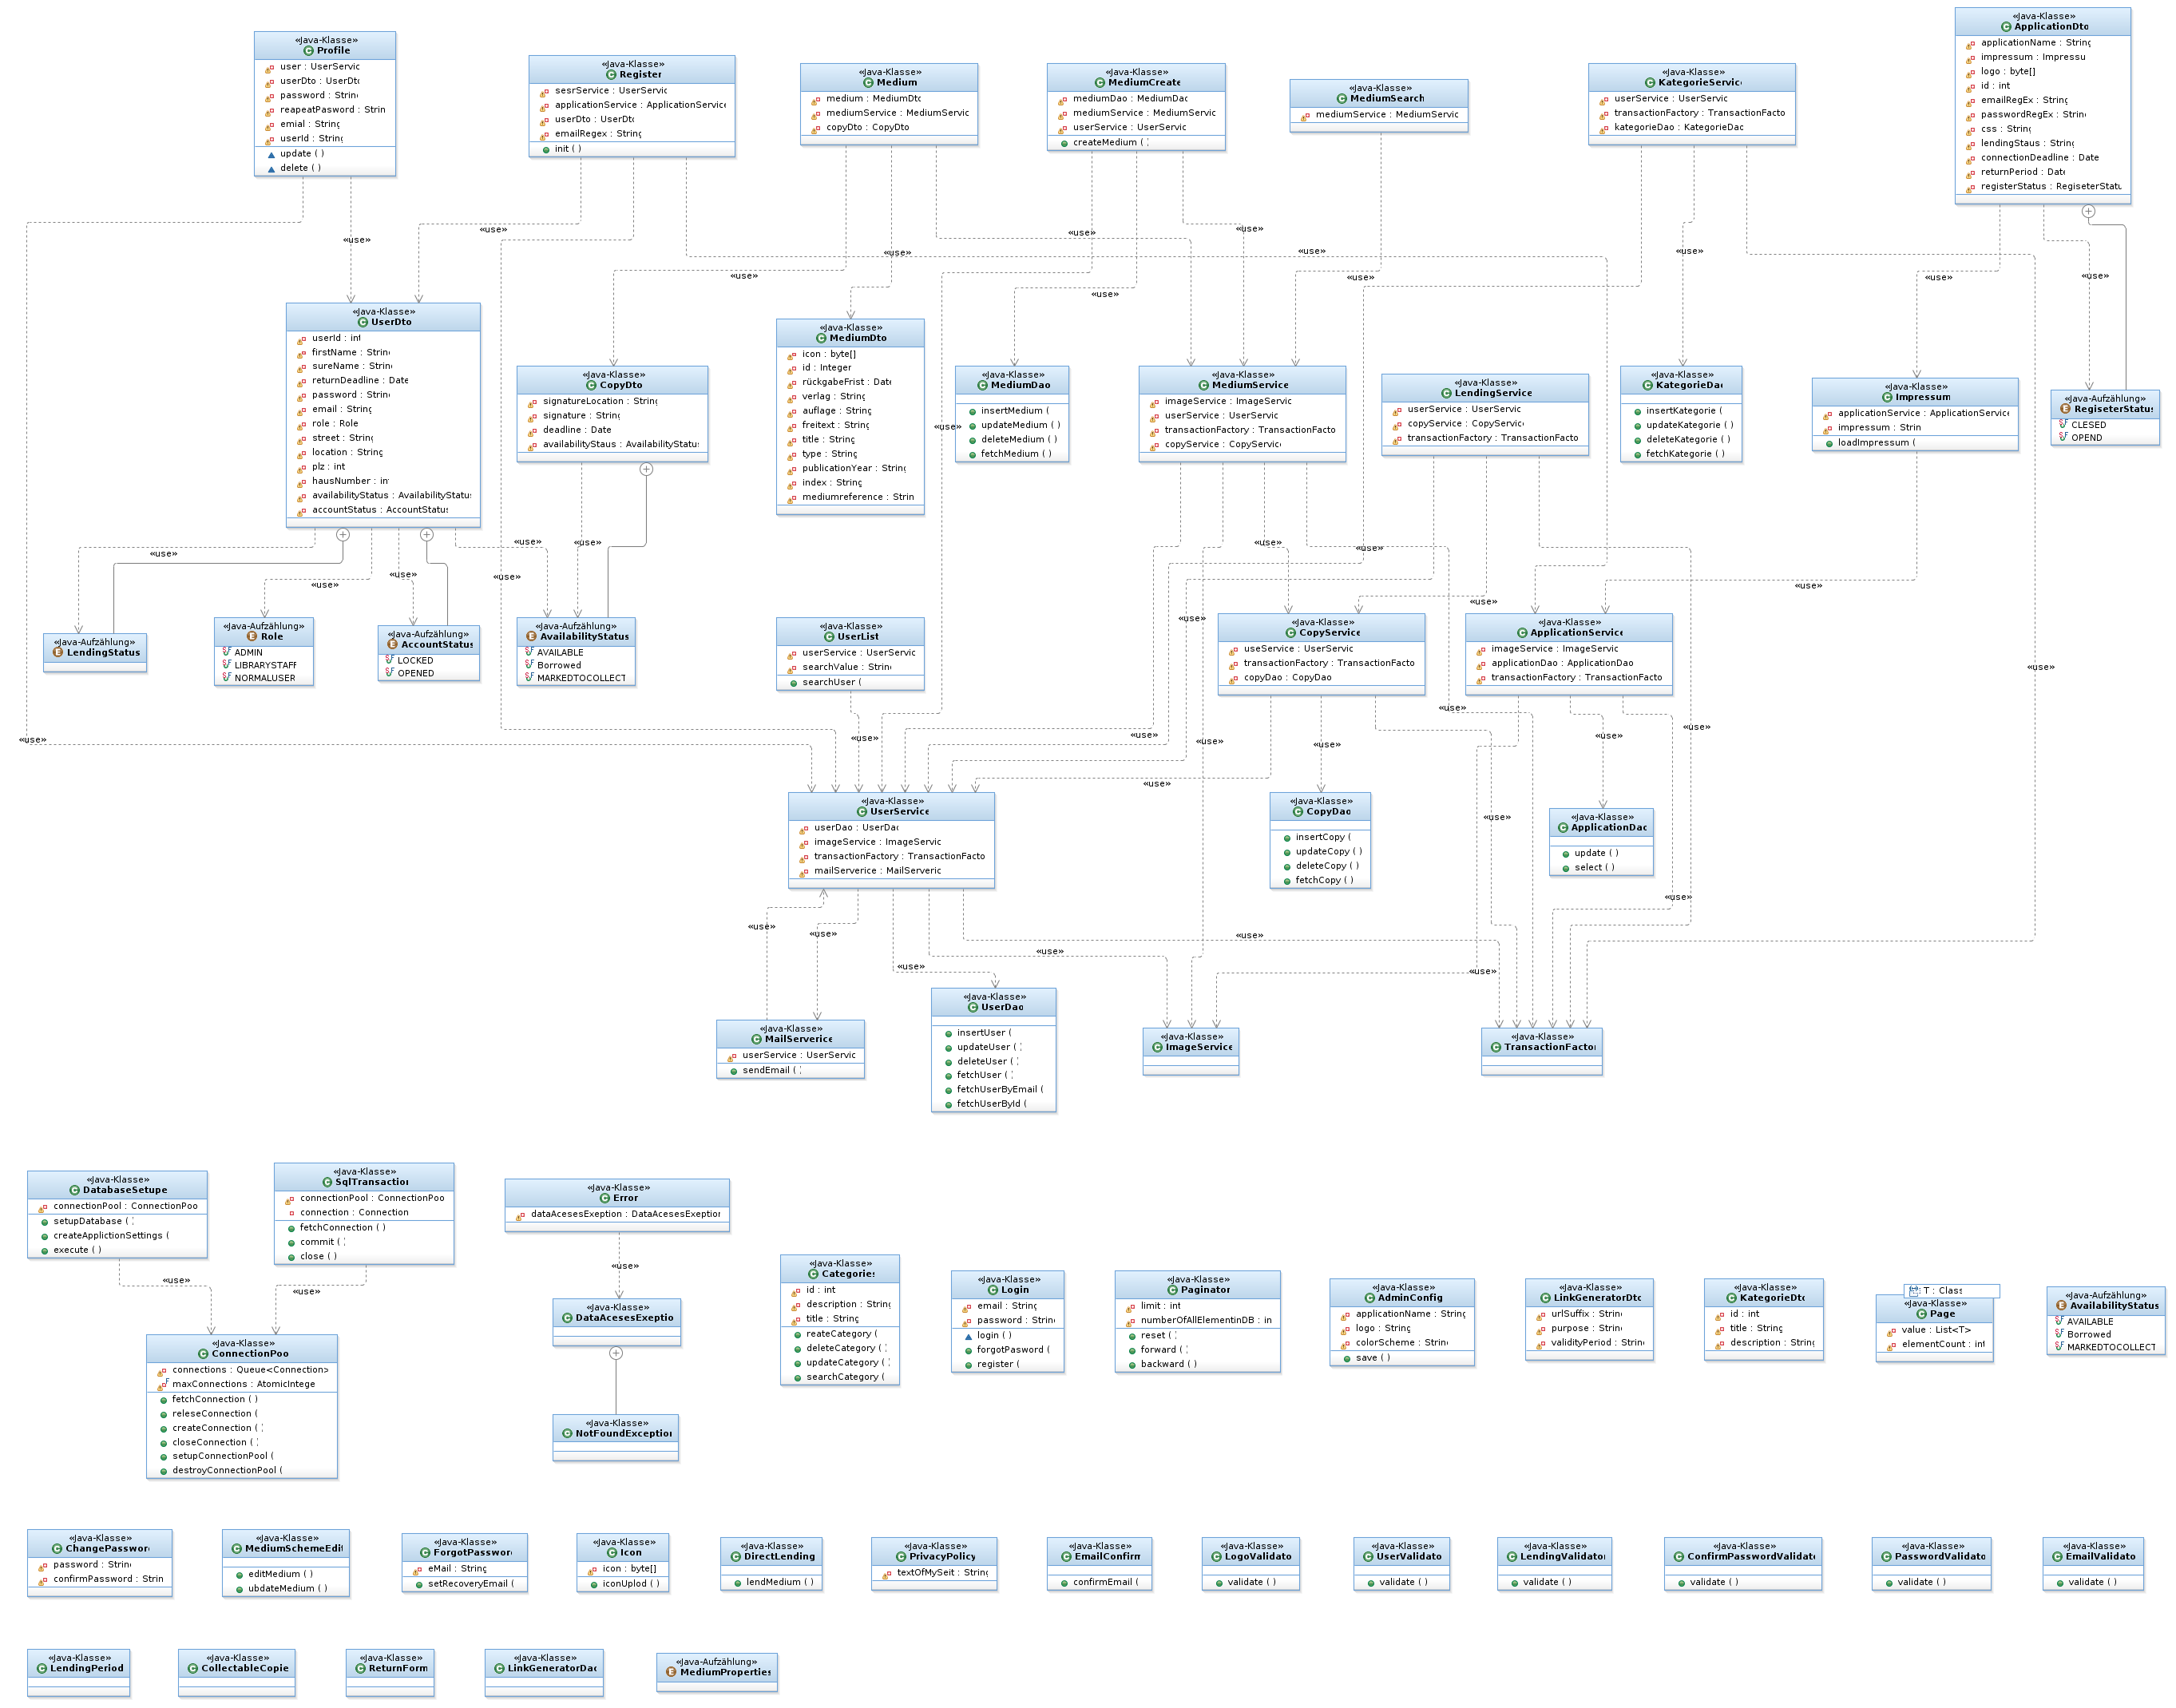
\includegraphics[scale=0.2]{Klassendiagramm.png}
        \caption{Klassendiagramm}
        \label{fig:Klassendiagramm}
    \end{figure}
%    \end{landscape}

%    \begin{landscape}
    \begin{figure}[H]
        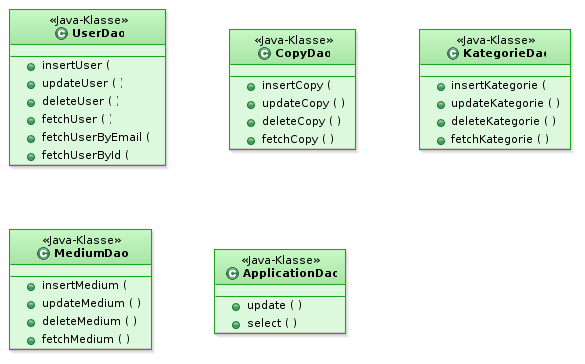
\includegraphics[scale=0.6]{KlassendiagramDao.png}
        \caption{Klassendiagramm der Daos}
        \label{fig:KlassendiagramDao}
    \end{figure}
%    \end{landscape}

%    \begin{landscape}
    \begin{figure}[H]
    \centering
        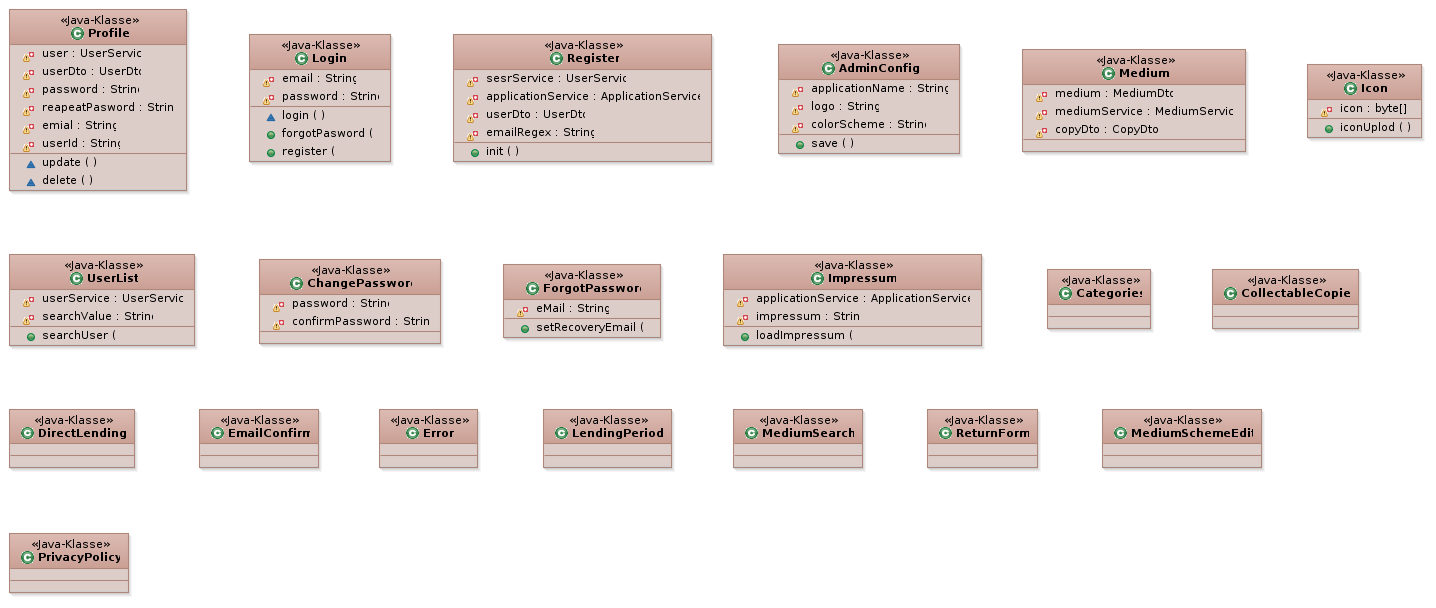
\includegraphics[scale=0.7, angle=270]{KlassendiagramBeans.png}
        \caption{Klassendiagramm der Beans}
        \label{fig:KlassendiagramBeans}
    \end{figure}
%    \end{landscape}

%    \begin{landscape}
    \begin{figure}[H]
        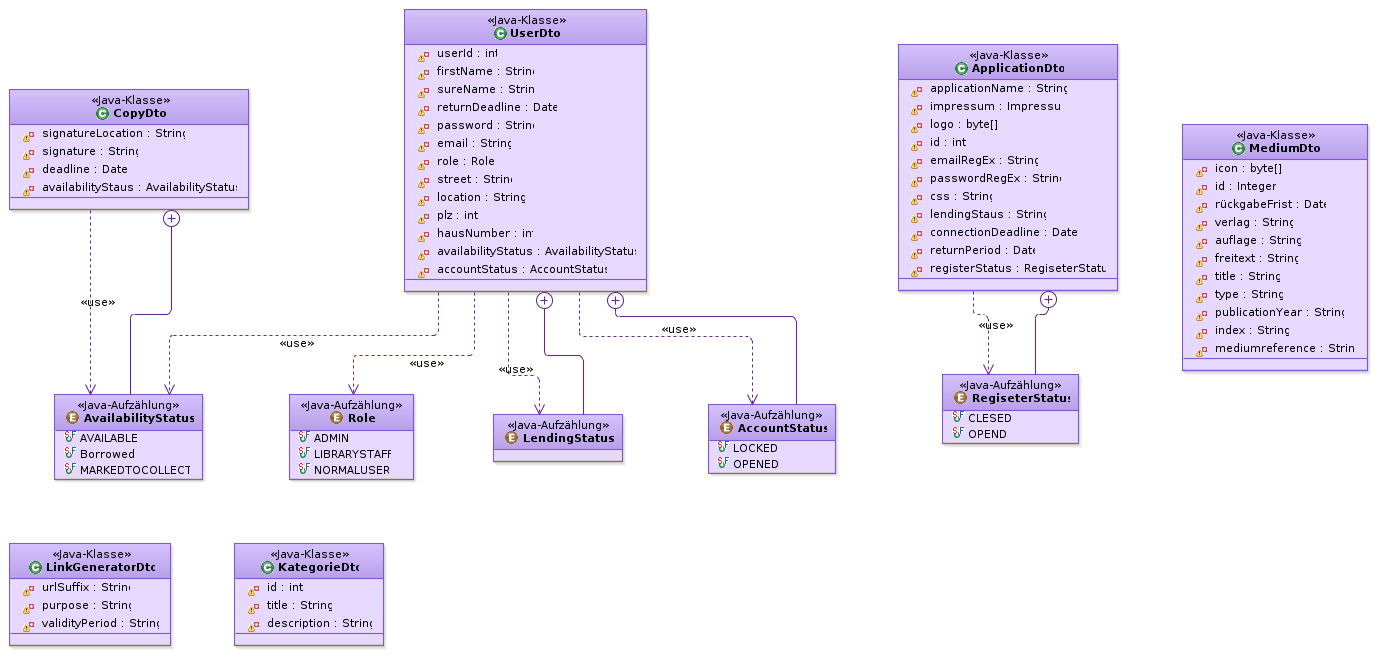
\includegraphics[scale=0.6]{KlassendiagramDtos.png}
        \caption{Klassendiagramm der Dtos}
        \label{fig:KlassendiagrammDto}
    \end{figure}
%    \end{landscape}


%    \begin{landscape}
    \begin{figure}[H]
        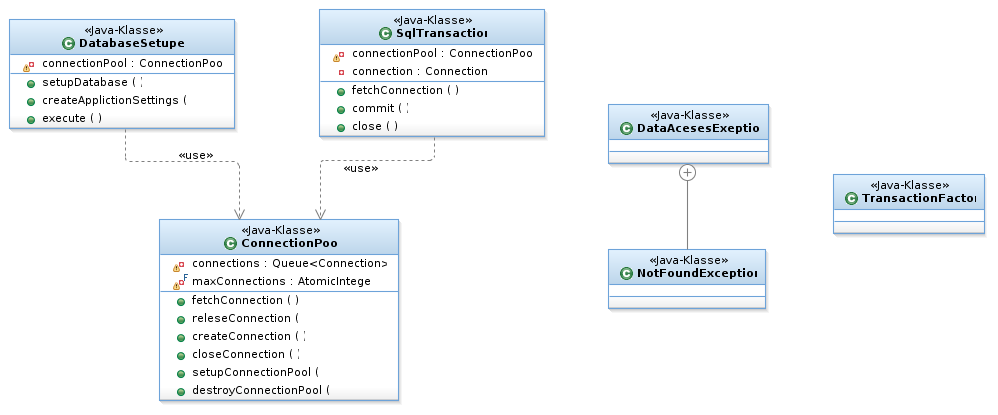
\includegraphics[scale=0.6]{KlassendiagramSystem.png}
        \caption{Klassendiagramm des Systems}
        \label{fig:KlassendiagramSystem}
    \end{figure}
%    \end{landscape}

%    \begin{landscape}
    \begin{figure}[H]
        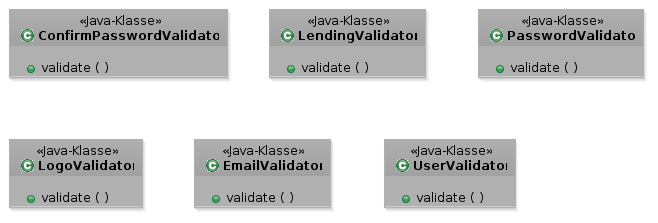
\includegraphics[scale=0.6]{klassendiagramValidator.png}
        \caption{Klassendiagramm des Validator}
        \label{fig:KlassendiagramValidator}
    \end{figure}
%    \end{landscape}


%   \begin{landscape}
    \begin{figure}[H]
        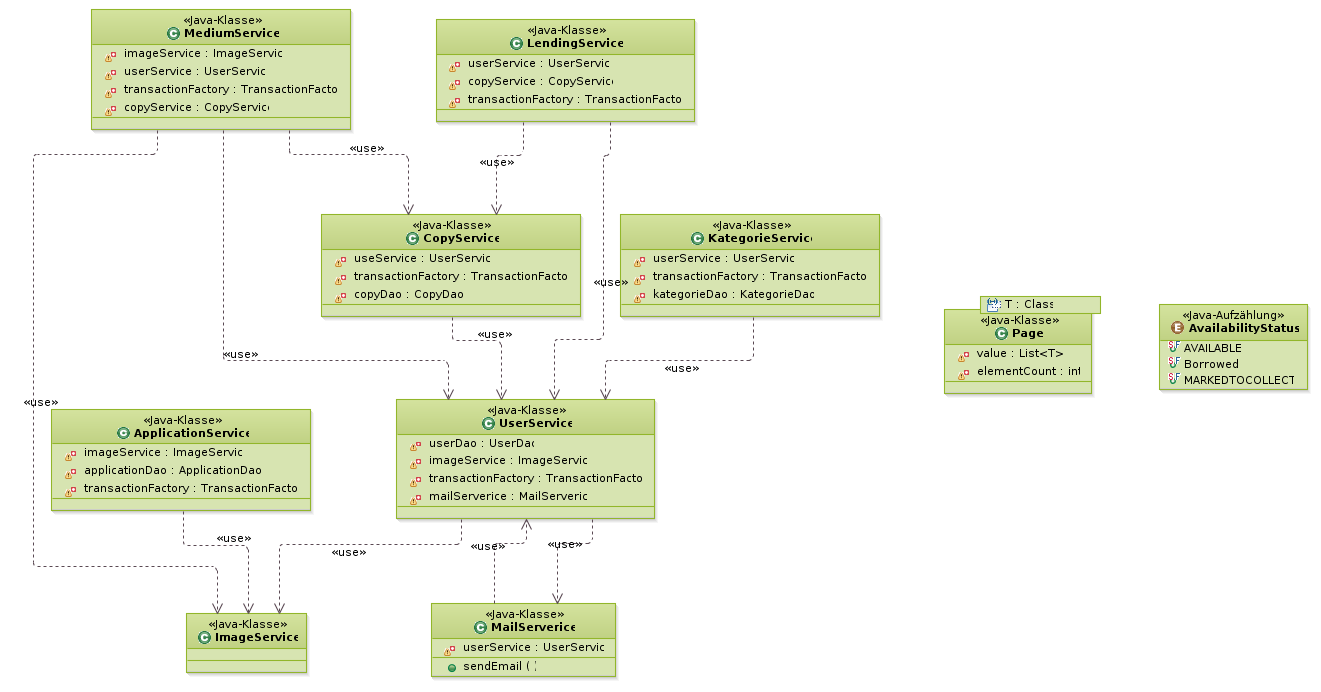
\includegraphics[scale=0.6]{KlassendiagramService.png}
        \caption{Klassendiagramm der Services}
        \label{fig:KlassendiagramService}
    \end{figure}
%    \end{landscape}



 \begin{center}
    \begin{table}
        \begin{tabular} { |p{3,5cm}|p{7,5cm}| }
            \hline
            Java-Klasse & Beschreibung  \\
            \hline\hline
            Medium & Backing Bean für das Erstellen und Bearbeiten eines Medium. \\
            \hline
            AdminConfig & Backing Bean für die Einstellung der Webseite. \\
            \hline
            ChangePassword & Backing Bean für die Änderung des Passwortes. \\
            \hline
            Error & Backing Bean der Seite die Fehlermeldungen anzeigt.\\
            \hline
            Profile & Backing Bean für das Anzeigen und Bearbeiten des Profils eines Benutzers. \\
            \hline
            ForgotPassword & Backing Bean für die Seite, auf der man sich einen neues Passwort zusenden lassen kann, wenn man das altes Passwort vergessen hat. \\
             \hline
            Login & Backing Bean des Logins. \\
             \hline
            Register & Backing Bean für das Anlegen eines neuen Benutzers. \\
            \hline
            Icon & Backing Bean für das Hochladen und Bearbeiten eines Mediums und Logo des Systems. \\
            \hline
            Category & Backing Bean für die Kategorie, die als Liste angezeigt wird. \\
            \hline
            UserList & Backing Bean für die Seite der Benutzersuche. \\
            \hline
            CollectableCopies & Backing Bean der Seite, auf der alle Exemplare abzuholend makiert. \\
            \hline
            DirectLendin & Backing Bean für die Seite der Directausleihe. \\
             \hline
            EmailConfirm & Backing Bean für die Seite der Emailbestätigung. \\
             \hline
            LendingPeriod & Backing Bean für die Seite der Ausleihefrist. \\
             \hline
            MediumSearch & Backing Bean für die Seite der Mediumsuche. \\
             \hline
            ReturnForm & Backing Bean für die Seite der Rückgabe. \\
             \hline
            MediumEdit & Backing Bean für die Seite des Mediumedieren. \\
             \hline
            PrivacyPolicy & Backing Bean für die Seite der Datenschutzerklärung. \\
            \hline
        \end{tabular}
        \end{table}
        \end{center}


\begin{center}
    \begin{table}
        \begin{tabular} { |p{3,5cm}|p{7,5cm}| }
            \hline
            Java-Klasse & Beschreibung  \\
             \hline\hline
            UserDto & Enthält alle Daten des Profils eines Benutzers. \\
            ApplicationDto & Enthält die Daten der Anwendung. \\
            \hline
            MediumDto & Enthält die Daten eines Mediums. \\
            \hline
            CopyDto & Enthält die   Daten eines Exemplar. \\
            \hline
            CategoryDto & Enthält die Daten einer Kategorie. \\
            \hline
            LinkGeneratorDto & Enthält die Daten des Linkgenerators. \\
            \hline
        \end{tabular}
        \end{table}
        \end{center}


  \begin{center}
    \begin{table}
        \begin{tabular} { |p{3,5cm}|p{7,5cm}| }
             \hline
            Java-Klasse & Beschreibung \\
            \hline\hline
            MediumDao & Kontrolliert den Zugriff auf Mediumdaten in der Datenbank. \\
             \hline
            ApplicationDao & Kontrolliert den Zugriff auf die Einstellungen der Anwendung, die in der Datenbank gespeichert sind. \\
            \hline
            UserDao & Kontrolliert den Zugriff auf Benutzerdaten in der Datenbank. \\
            \hline
            CategoryDao & Kontrolliert den Zugriff auf Kategoriedaten in der Datenbank. \\
            \hline
            CopyDao & Kontrolliert den Zugriff auf die Exemplardaten in der Datenbank. \\
            \hline
        \end{tabular}
        \end{table}
        \end{center}


  \begin{center}
    \begin{table}
        \begin{tabular} { |p{3,5cm}|p{7,5cm}| }
             \hline
            Java-Klasse & Beschreibung  \\
           \hline\hline
            EmailValidator & Prüft ob es sich eine gültige E-Mail-Adresse handelt. \\
            \hline
            PasswordValidator & Prüft beim Anlegen eines neuen Benutzerkontos oder beim Ändern des Passwortes, ob das Passwort den Mindestanforderungen entspricht. \\
             \hline
            ConfirmPasswordValidator & Prüft ob die Passwortbestätigung und Passwort übereinstimmen. \\
            \hline
           LogoValidator & Validiert ob eine Datei einem gängigen Bildformat entspricht und nicht zu groß oder auch zu klein ist. \\
             \hline
            UserValidator & Prüft ob eine Ausleihe deren Frist abgelaufen ist. \\
            \hline
            LendingValidator & Prüft ob eine Ausleihe deren Frist abgelaufen ist. \\
            \hline
        \end{tabular}
        \end{table}
        \end{center}


  \begin{center}
    \begin{table}
        \begin{tabular} { |p{3,5cm}|p{7,5cm}| }
              \hline
            Java-Klasse & Beschreibung  \\
           \hline\hline
            ConnectionPool & Verwaltet die Verbindungen zur Datenbank. \\
            \hline
            DatabaseSetup& Erstellt das Datenbankschema und die Verbindung mit Datenbank. \\
             \hline
            SqlTransaction& Wird verwendet, um eine Sql-Transaction zu verarbeiten. \\
             \hline
            DataAcesesException& Wird geworfen,  wenn es keine Verbindung mit Datenbank gibt. \\
           \hline
        \end{tabular}
        \end{table}
        \end{center}


     \begin{center}
       \begin{table}
        \begin{tabular} { |p{3,5cm}|p{7,5cm}| }
             \hline
            Java-Klasse & Beschreibung \\
            \hline\hline
            MediumService &  Service für Aktionen zu Medien. \\
             \hline
            ApplicationService & Service für Aktionen zu der Anwendung. \\
            \hline
            UserService & Service für Aktionen zu dem Benutzer des System. \\
            \hline
            CategoryService & Service für Aktionen zu Kategorie. \\
            \hline
            CopyService& Service für Aktionen zu Exemplaren.\\
             \hline
           LendingService & Service für Aktionen zu der Ausleihe. \\
           \hline
        \end{tabular}
        \end{table}
        \end{center}

\subsection{Paketdiagramm}

    \begin{figure}[h!]
        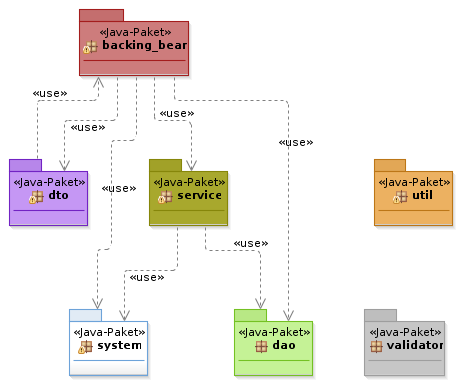
\includegraphics[scale=0.6]{Paketdigram.png}
        \caption{Paketdiagramm}
        \label{fig:Paketdiagramm}
    \end{figure}




%--JSF-Dialoge-----------------------------------------------------------------------------------------------------------------------------------------------------------------------
\section{JSF-Facelets}
\sectionauthor{León Liehr}

% TASK add javadocs
% TASK update AJAX note
% TASK mention query strings and GET/POST parameters!!

\newcommand{\PUB}{jeder}
\newcommand{\ANO}{Anon.}
\newcommand{\USR}{Nutzer}
\newcommand{\BIB}{Mitarbeiter}
\newcommand{\ADM}{Admin.}

\newcommand{\component}[2]{\subsubsection{#1 (\texttt{#2})}}
\newcommand{\page}[2]{
    \subsubsection{#1}
    \paragraph*{Dateipfad} \texttt{#2.xhtml}
}

\newcommand{\Javadoc}{\paragraph*{Javadoc}}

\newcommand{\BTN}{Knopf}
\newcommand{\LNK}{Hyperlink}
\newcommand{\INP}{Eingabefeld}
\newcommand{\PAS}{Passworteingabefeld}
\newcommand{\DRP}{Drop-Down-Liste}
\newcommand{\CHK}{Checkbox}
\newcommand{\OUT}{Ausgabefeld}
\newcommand{\LST}{Paginierte Liste}

\newenvironment{controls}
{
    \begin{table}[H]
        \centering
        \begin{tabular}{ p{7em} p{25em} p{7em} }
            \toprule
            \textbf{Typ} & \textbf{Beschreibung} & \textbf{Sichtbarkeit}\\
            \midrule
        }
        {
            \bottomrule
        \end{tabular}
    \end{table}
}

Sofern nicht anders ausgewiesen folgt jedem Eingabefeld und \PAS ein Ausgabefeld für Meldungen (genauer gesagt eine JSF-\texttt{HtmlMessage}-Komponente), insb. für von JSF-Validatoren geworfene Fehlermeldungen.

% Frage: sind diese Eingabefelder für E-Mails benutzerdef. Komponenten?
% Aufgabe schau dir das Kap zu AJAX im Buch an!!
Aufbauend auf der Voraussetzung einer modernen JavaScript-Implementierung in dem Webbrowser des Clients (Pflichtenheft, Abschnitt 4.1) wird bei Eingabefeldern für E-Mail-Adressen (MANCHER), Signaturen (MANCHER) und Standorten (MANCHER) statt der überholten AJAX-Technologie\footnote{\url{https://xhr.spec.whatwg.org/}} die sog. Fetch API\footnote{\url{https://fetch.spec.whatwg.org/}} verwendet, um während der Eingabe Vorschläge von existierenden Einträgen einblenden zu können.

Mit dem Elementtyp Eingabe wird im Folgenden JSFs \texttt{ui:insert} gemeint.

Zudem werden nachfolgend diese Abkürzungen und Kurzformen verwenden:

% TASK inline table
\begin{table}[H]
\centering
\begin{tabulary}{\textwidth}{RL}
\toprule
%\PUB & jeder \\
\ANO  & Anonymus \\
\USR & angemeldeter Nutzer \\
\BIB & Bibliotheksmitarbeiter \\
\ADM & Administrator \\
\bottomrule
\end{tabulary}
\end{table}

\subsection{Komponenten}

\component{\LST}{PaginatedList}

% TASK attributes, values

\begin{controls}
    \BTN & zum Blättern auf die nächste Seite & \PUB\\
    \BTN & zum Blättern auf die vorige Seite & \PUB\\
    ?? & ?? values & \\
    \BTN & ?? SORT SPECIFIC COLUMN (asc/desc) & \PUB\\
    \OUT & INFO WHERE WE ARE & \PUB\\
\end{controls}

\component{Editierbarer Text}{EditableText}

Das Attribut der Komponente ist der Text.

% QUESTION visibility as an attribute, too?? if yes, how???

\begin{controls}
    \OUT & für das Textattribut & \PUB\\
    \INP & für das Textattribut & \ADM\\
\end{controls}

\subsection{Seitenvorlagen (Templates)}

\page{Einzige Seitenvorlage}{public/template}\label{template}

\begin{controls}
    Einlage & des Titels einer konkreten Seite & \PUB\\
    Einlage & des Inhalts einer konkreten Seite & \PUB\\
    \BTN & zum Anzeigen der kontextsensitiven Hilfe; als Fragezeichenbildsymbol dargestellt & \PUB\\
    \LNK & zu der erweiterten Suche & \PUB\\
    \INP & für die Mediensuche; alleinig die Betätigung der Eingabetaste sendet ab & \PUB\\
    \LNK & zu der Profilseite & \USR\\
    \LNK & zum Abmelden; zur Anmeldemaske & \USR\\
    \LNK & zur Anmeldemaske & \ANO\\
    \LNK & zur Registrierungsseite  & \ANO\\
    \LNK & zu den abzuholenden Exemplaren & \BIB\\
    \LNK & zu der Medienrückgabe & \BIB\\
    \LNK & zu der Direktausleihe & \BIB\\
    \LNK & zu der Medienerstellung & \BIB\\
    \LNK & zu der Verwaltung & \ADM\\
    \OUT & für globale Meldungen (JSFs \texttt{HtmlMessages}) & \PUB\\
    \LNK & zur Datenschutzerklärung & \PUB\\
    \LNK & zum Impressum & \PUB\\
    \LNK & zum Kontakt & \PUB\\
\end{controls}

\subsection{Seiten}

Alle Seiten nehmen die einzige Seitenvorlage (\ref{template}) als Vorlage.
Jede Seite wird vom einer entsprechenden Backing Bean angetrieben, welche sich namentlich lediglich durch die Schreibweise unterscheidet. So wird bspw. die Seite \texttt{privacy-policy.xhtml} (in \textit{dash case}) mit der Bean \texttt{PrivacyPolicy} (in \textit{upper camel case}) assoziiert.

\page{Abzuholende Exemplare}{staff/copies-ready-for-pickup}

\Javadoc
This page is used by library staff to be up to speed regarding which copies are ready to be picked up and
whether they can expect someone to soon enter the library and arrive at their counter.

\begin{controls}
    \LST & aller abzuholenden Exemplare & \BIB\\
\end{controls}

\page{Eigene abzuholende Exemplare}{account/my-copies-ready-for-pickup}

\Javadoc
On this page a user gets to know which copies they want to pick up from the library and borrow thereafter
and how much time they have left to do so until they exceed the deadline.

\begin{controls}
    \LST & aller abzuholenden Exemplare & \USR\\
\end{controls}

\page{Eigene ausgeliehene Exemplare}{account/my-borrowed-copies}

\Javadoc
This page informs the user which copies they borrowed from the library and how much time they still have left
until they have to return them to not exceed the deadline.

\begin{controls}
    \LST & aller ausgeliehenen Exemplare & \USR\\
\end{controls}

\page{Anmeldemaske}{public/login}

\Javadoc
This page is the one users first face when they are not already logged in.
It allows them to log into the system to gain the privilege to borrow copies.
If a logged-in user accesses this page by manually entering its URL, a message is shown instead of the
login form and they get automatically redirected to their profile page.

\begin{controls}
    \INP & für die E-Mail-Adresse & \ANO\\
    \PAS & & \ANO\\
    \BTN & zum Anmelden & \ANO\\
    \BTN & zum Passwortzurücksetzen; als \LNK dargestellt, um unauffälliger zu sein, da es eine zweitrangige Aktion ist & \ANO\\
\end{controls}

\page{Datenschutzerklärung}{public/privacy-policy}

\Javadoc
This page declares the privacy policy of this system.

\begin{controls}
    \OUT & für die Datenschutzerklärung & Nicht-\ADM\\
    \INP & für die Datenschutzerklärung & \ADM\\
    \BTN & zum Speichern der Änderungen & \ADM\\
\end{controls}

\page{Direktausleihe}{staff/direct-lending}

\Javadoc
This page enables staff to lend a person most probably in front of their counter a series of copies.
It is intended but not a hard requirement that library staff scans the copies given to them by the customer with a dedicated device which automatically pastes the signatures into the relevant input fields. Analogously with the email address stored inside of their membership card.

\begin{controls}
    \INP & für die E-Mail-Adresse des Ausleihenden & \BIB\\
    \INP & für die Signatur eines auszuleihenden Exemplars; beim Laden der Seite fünfmal vorhanden. Durch das Pressen des relevanten Knopfs wird ein weiteres Feld angehängt & \BIB\\
    \BTN & zum Hinzufügen eines weiteren Signaturfelds & \BIB\\
    \BTN & zum Ausleihen & \BIB\\
\end{controls}

\page{E-Mail-Bestätigung}{public/email-confirmation}

\Javadoc
Accessing this page potentially verifies the email address of a specific user. For this,
it takes a token as a query parameter. If absent or invalid, nothing user-facing happens.
This secures against certain attacks.

\page{Fehlerseite}{public/error}

\Javadoc
The sink for all kinds of fatal errors that happened in the system.
They are either caused client-side (HTTP status codes 4XX) or server-side (HTTP status codes 5XX).
If it's a client-side error, the user gets redirected to either the login page or their profile depending on if they are logged in or not. The redirection happens after some fixed amount of time.

\begin{controls}
    \OUT & für den Titel der Fehlermeldung & \PUB\\
    \OUT & für die Beschreibung des Fehlers & \PUB\\
\end{controls}

\page{Impressum}{public/site-notice}

\Javadoc
This page contains the site notice.

\begin{controls}
    \OUT & für das Impressum & Nicht-\ADM\\
    \INP & für das Impressum & \ADM\\
    \BTN & zum Speichern der Änderungen & \ADM\\
\end{controls}

\page{Kategorienbearbeitung}{staff/category-editor}

% Task: rephrase
\Javadoc The category editor allows the creation and modification of a category.
Generally this page is accessed from the category browser
This page can be reached when library staff clicks on the edit button next to a category's name in the browser.
In this case, the identifier of the category to be edited is transmitted as a parameter.
This page can be reached when library staff clicks on the create button in the context of a category.
In that case, the identifier of the category to be treated as the parent of the new category is transmitted
as a parameter.
If the parameters are invalid, the user will be redirected to the error page.

\begin{controls}
    \INP & für den Kategorienamen & \BIB\\
    \INP & für die Kategoriebeschreibung & \BIB\\
    \BTN & zum Speichern der Änderungen & \BIB\\
\end{controls}

\page{Kategorierenstöberer}{public/category-browser}

\Javadoc
This page offers users to browse through all available categories mediums are part of in a structured manner.
It renders it possible for the consumer to discover new mediums.

\begin{controls}
    \INP & für den Suchterm der Kategoriensuche & \PUB\\
    \BTN & zum Durchführung der Suche & \PUB\\
    Baumansicht \ref{treeview} & mancher Kategorien & \PUB\\
    \LNK & zur Kategorienbearbeitung (Erstellung einer neuen) & \BIB\\
    \LNK & zur Kategorienbearbeitung & \BIB\\
    \BTN & zum Löschen der Kategorie; zur Elterkategorie & \BIB\\
    \LNK & zur Medienerstellung unter der aktuellen Kategorie & \BIB\\
\end{controls}

% TASK BEACON !!!!

\begin{table}[H]
    \centering
    \begin{tabular}{ p{6em} p{6em} p{19em} p{7em} }
        \toprule
        \midrule
        \bottomrule
    \end{tabular}
    \caption{Baumansicht}
    \label{treeview}
\end{table}

\page{Kontakt}{public/contact}

\Javadoc The contact page allows any user to get to know how to contact the site owners.

\begin{controls}
    \OUT & für die Kontaktinformationen & Nicht-\ADM\\
    \INP & für das Kontaktinformationen & \ADM\\
    \BTN & zum Speichern der Änderungen & \ADM\\
\end{controls}

\page{Leihfristverstöße}{admin/lending-period-violations}

\Javadoc
XXX

\begin{controls}
    \LST & von Exemplaren und Nutzern & \ADM\\
\end{controls}

\page{Medienerstellung}{staff/medium-creation}

\Javadoc
XXX

\begin{controls}
    \INP & für ein Medienattribut; existiert pro Medienattribut & \BIB\\
    \INP & für die Rückgabefrist & \BIB\\
    \INP & für den Standort eines neuen Exemplars & \BIB\\
    \INP & für die Signatur eines neuen Exemplars & \BIB\\
    \BTN & zum Anlegen des neuen Mediums und des ersten Exemplars & \BIB\\
\end{controls}

\page{Medienrückgabe}{staff/return}

\Javadoc
XXX

\begin{controls}
    \INP & für die E-Mail-Adresse des Kunden & \BIB\\
    \INP & für die Signatur eines abzugebenden Exemplars; beim Laden der Seite fünfmal vorhanden & \BIB\\
    \BTN & zum Hinzufügen eines weiteren Signaturfelds & \BIB\\
    \BTN & zum Abgeben & \BIB\\
\end{controls}

\page{Mediensuche}{public/media-search}

\Javadoc
This page permits users to search for mediums given some of their attributes as search criteria.
Further, a user can search mediums by category and by the signature of one of their copies.
The page has an optional query parameter corresponding to the search term.
If it is not provided, nothing will be searched and the paginated list of results will not be displayed at all.

\begin{controls}
    \INP & für den Suchterm der freien Suche & \PUB\\
    \BTN & zur Durchführung der Suche & \PUB\\
    \DRP & für den Suchoperator; beim Laden der Seite dreimal vorhanden (je gruppiert mit Suchkriterium und -feld) & \PUB\\
    \DRP & für das Suchkriterium; beim Laden der Seite dreimal vorhanden (je gruppiert mit Suchoperator und -feld) & \PUB\\
    \INP & für den Suchterm der differenzierten Suche; beim Laden der Seite dreimal vorhanden (je gruppiert mit Suchoperator und -kriterium) & \PUB\\
    \BTN & zum Hinzufügen eines weiteren Gruppe aus Suchoperator, -kriterium und -feld & \PUB\\
    \LST & aller Suchergebnisse; nur sichtbar, wenn schon gesucht wurde & \PUB\\
\end{controls}

\page{Mediumsansicht}{public/medium}

\Javadoc
XXX

\begin{controls}
    \LNK & zurück zur Trefferliste / Mediensuche; nur sichtbar, falls der Nutzer von der Suche kommt & \PUB\\
    \OUT & für ein Medienattribut; existiert pro Medienattribut; mehrwertige Attribute durch Komma getrennt angezeigt & \ANO, \USR\\
    \INP & für ein Medienattribut; existiert pro Medienattribut bzw. pro Wert bei mehrwertigen & \BIB\\
    \BTN & zum Speichern der Änderungen an den Medienattributen & \BIB\\
    \BTN & zur Bindung an die Abholung des Mediums; nur sichtbar, falls es dem Nutzer erlaubt ist auszuleihen & \USR\\
    \OUT & für die Rückgabefrist; bezieht auch die nutzerbezogene Frist ein, anders als das \INP{} darunter & \USR\\
    \INP & für die Rückgabefrist & \BIB\\
    \BTN & zum Speichern der Änderungen an der Rückgabefrist & \BIB\\
    \LNK & zum Löschen des Mediums; zur zuvor aufgerufenen Seite & \BIB\\
    Tabelle \ref{tableofcopies} & aller Exemplare & \PUB\\
    \INP & für den Standort eines neuen Exemplars & \BIB\\
    \INP & für die Signatur eines neuen Exemplars & \BIB\\
    \BTN & zum Erstellen eines Exemplars & \BIB\\
\end{controls}

% TASK param given to actions
% TASK JSF DataTable
% QUESTION sorting???

\begin{table}[H]
    \centering
    \begin{tabular}{ p{6em} p{6em} p{19em} p{7em} }
        \toprule
        \textbf{Spalte} & \textbf{Typ} & \textbf{Beschreibung} & \textbf{Sichtbarkeit}\\
        \midrule
        Standort & \OUT & & \PUB\\
        Standort & \INP & & \BIB\\
        Verfügbarkeit & \OUT & & \PUB\\
        Signatur & \OUT & & \PUB\\
        Signatur & \INP & & \BIB\\
        Aktionen & \BTN & zum Speichern der Änderungen & \BIB\\
        Aktionen & \BTN & zum Löschen & \BIB\\
        Aktionen & \BTN & zum Stornieren einer Abholung & \BIB\\
        Aktionen & \LNK & zur Direktausleihe & \BIB\\
        Aktionen & \BTN & zur Bindung an die Abholung; nur sichtbar, falls es dem Nutzer erlaubt ist auszuleihen & \USR\\
        \bottomrule
    \end{tabular}
    \caption{Tabelle aller Exemplare. Jede Zeile existiert pro Exemplar}
    \label{tableofcopies}
\end{table}

\page{Mediumschemabearbeitung}{admin/medium-schema-editor}

\Javadoc
On this page, the administrator can adjust the medium schema (the set of attributes of each medium).

\begin{controls}
    \INP & für den Namen eines Attributs; existiert pro Attribut & \ADM\\
    \DRP & für den Typen eines Attributs; existiert pro Attribut & \ADM\\
    \DRP & für die Position in der Medienvorschau; existiert pro Attribut & \ADM\\
    \BTN & zum Löschen eines Attributes; existiert pro Attribut & \ADM\\
    \BTN & zum Hinzufügen eines weiteren Gruppe aus \INP{}ern und \DRP{}n & \ADM\\
    \BTN & zum Speichern der Änderungen & \ADM\\
\end{controls}

\page{Nutzersuche}{admin/user-search}

\Javadoc
This page enables administrators to search for users.
The page has an optional query parameter corresponding to the search term.
If it is not provided, nothing will be searched and the paginated list of results will not be displayed at all.

\begin{controls}
    \INP & für den Suchterm & \ADM\\
    \BTN & zur Durchführung der Suche & \ADM\\
    \CHK & für das Einschränken auf gesperrte Nutzer & \ADM\\
    \LST & aller Suchergebnisse; nur sichtbar, wenn schon gesucht wurde & \ADM\\
\end{controls}

\page{Passwortzurücksetzung}{public/password-reset}

%TASK rephrase
\Javadoc
This page is reached by a user when they click on the link they received in an email.
For the mechanisms to work, it takes a token as a query parameter.
After submitting the form, the user is not logged into the system yet, they are redirected to the login form.
This secures against certain attacks.
If the token is absent or invalid, nothing user-facing will happen: Clicking the button still means redirection to the login page.

\begin{controls}
    \PAS & für das neue Passwort & \PUB\\
    \PAS & zur Bestätigung des neuen Passworts & \PUB\\
    \BTN & zum Zurücksetzen des Passworts; zur Anmeldemaske & \PUB\\
\end{controls}

\page{Profilseite}{account/profile}

% expand
\Javadoc
This page is either the profile page of the current user or if it is an administrator possibly also
of a user different from the logged-in one.
It allows a user to change their personal information the system stores and it allows administrators to manage other accounts.

\begin{controls}
    % BEACON TASK BEACON \INP_OR_OUT (new component)
    \INP & für den Vornamen & \USR\\
    \INP & für den Nachnamen & \USR\\
    \PAS & für das Passwort & \USR\\
    \PAS & zur Bestätigung & \USR\\
    \INP & für die E-Mail-Adresse & \USR\\
    \INP & für den Ort & \USR\\
    \INP & für die PLZ & \USR\\
    \INP & für die Straße& \USR\\
    \INP & für die Hausnummer & \USR\\
    \DRP & für die Nutzerrolle & \ADM\\
    \CHK & zum Sperren des Nutzers & \ADM\\
    \INP & für die Rückgabefrist & \ADM\\
    \BTN & zum Speichern der Änderungen an den Benutzerdaten & \USR\\
    \LNK & zu den abzuholenden und ausgeliehenen Exemplaren & \USR\\
    \BTN & zum Schließen des Accounts; zur Anmeldemaske & \USR\\
    \BTN & zum Löschen des Nutzers; zur Verwaltungsseite & \ADM\\
\end{controls}

\page{Registrierungsseite}{public/registration}

\Javadoc
On this page an anonymous user can register themself. Additionally, it can be used by administrators to register new users.

\begin{controls}
    \INP & für den Vornamen & \ANO/\ADM\\
    \INP & für den Nachnamen & \ANO/\ADM\\
    \PAS & & \ANO/\ADM\\
    \PAS & zur Bestätigung & \ANO/\ADM\\
    \INP & für die E-Mail-Adresse & \ANO/\ADM\\
    \INP & für den Ort & \ANO/\ADM\\
    \INP & für die PLZ & \ANO/\ADM\\
    \INP & für die Straße & \ANO/\ADM\\
    \INP & für die Hausnummer & \ANO/\ADM\\
    \DRP & für die Nutzerrolle & \ADM\\
    \BTN & zum Registrieren des Accounts & \ANO/\ADM\\
\end{controls}

\page{Verwaltungsseite}{admin/administration}

\Javadoc
This page provides the means to administrators to change the global settings of the application.

\begin{controls}
    \INP & für die Rückgabefrist & \ADM\\
    \INP & für den Mahnungszeitpunkt & \ADM\\
    \INP & für die Abholfrist & \ADM\\
    \INP & für den Systemnamen & \ADM\\
    \CHK & für den Zugangsstatus (anonym oder nicht) & \ADM\\
    \CHK & für den Registrierungsstatus & \ADM\\
    \INP & für den regulären Ausdruck valider E-Mail-Adressen & \ADM\\
    \DRP & für das Farbschema des Systems & \ADM\\
    Datei-Upload & für das Logo des Systems & \ADM\\
    \BTN & zum Speichern der Änderungen an den Systemeinstellungen & \ADM\\
    \LNK & zu der Registrierungsseite (fremden Nutzer erstellen) & \ADM\\
    \LNK & zur Mediumsschemabearbeitung & \ADM\\
    \LNK & zu den Leihfristverstößen & \ADM\\
    \LNK & zur Nutzersuche & \ADM\\
    \INP & für den Suchterm einer Nutzersuche & \ADM\\
    \BTN & zum Durchführung der Suche & \ADM\\
\end{controls}
 
%--Systemfunktionen----------------------------------------------------------------------------------------------------------------------------------------------------------------
\section{Systemfunktionen}
\sectionauthor{Jonas Picker}
\subsection{Technische Systemsicherheit}
\noindent \textbf{Kommunikationsverschlüsselung:} Durch die CA-Zertifizierung des Servers wird eine TLS-Trans-portverschlüsselung bei der Kommunikation zwischen Klient und Server verwendet. Ist die Datenbank, wie im Pflichtenheft (Abschnitt 4.3  'Server') beschrieben, über SSL-VPN angebunden, ist die Kommunikation zwischen ihr und dem Server ebenfalls verschlüsselt. \\
\textbf{Nutzerberechtigungen:} Für die Überprüfung der Zugangsberechtigungen bei jeder HTTPS-Anfrage implementiert die Klasse !!!\hyperlink{PhaseListener}{}!!! das PhaseListener-Interface, welches zu implementierende Methoden zum Ausführen von Code vor oder nach jeder Phase des JSF-Life-Cycle vorgibt. In unserem Fall wird am frühestmöglichen Punkt (vor der Restore-View-Phase) geprüft, ob der Anfragesteller auch berechtigt ist, die vorhergesehene Antwort vom Server zu erhalten. Aus Redundanzgründen verwenden wir für Seiten, auf die mehrere Nutzerrollen Zugriff haben, die gleichen Facelets. In den jeweiligen Backing-Beans wird dann, durch Zugriff auf die von JSF getrackte Nutzer-Session der Klasse !!!\hyperlink{Session}{}!!!, die Rolle des Benutzers überprüft. Für jeden Seitenbesucher werden dann nur die rollenspezifischen Knöpfe und Anzeigen gerendert (siehe Abschnitt !!!\hyperlink{Facelets}{JSF-Facelets}!!!). Durch die inklusive Rollenhierarchie lassen sich so alle Funktionalitäten der Rollen im gleichen Facelet einbinden.\\
\textbf{Session-Hijacking\footnote{Das Stehlen einer validen Nutzer-Session um Zugriff auf den Account und seine Berechtigungen zu erhalten}:} Um diesen Angriffsvektor zu schützen, wird der Identifikator der Nutzer-Session an kritischen Stellen (z.B. nach dem Login) manuell ausgetauscht. \\
\textbf{Cross-Site-Scripting\footnote{Auch XSS: das Einschleusen von browserinterpretierbarem HTML-Code auf ungesicherte Teile einer Website}:} Das Escapen von HTML-Sonderzeichen wird von JSF bei allen nutzergenerierten Teilen der Anwendung unterstützt. Alle Elemente der JSF-Facelets, die nutzergenerierten In- und Output weitergeben, haben den impliziten Standartwert 'escape=true'. Da wir diesen in unserer Implementierung nie manuell auf 'false' setzen, ist XSS in dieser Applikation unmöglich. \\
\textbf{SQL-Injection\footnote{Einschleusen von SQL-Code in Formularfelder, um Zugriff auf die Datenbank zu erhalten}:} Durch das Konsequente Verwenden der 'Prepared Statements' in unserer !!!\hyperlink{DAOs}{Datenzugriffsschicht}!!! beugen wir SQL-Injections vor. Diese JDBC-Funktionalität trennt das eigentliche SQL-Statement von den nutzergenerierten Parametern und Verhindern so das Ausführen von maliziösem SQL-Code in der Datenbank. \\
\subsection{Logging}
Mit der Klasse !!!\hyperlink{Logger}{Logger}!!! ist unser System mit einer eigenen Log-Funktion ausgestattet. Diese dient sowohl zum Debugging während der Entwicklung, als auch zum Protokollieren der Fehler und Abläufe im laufenden System. Durch Setzten der Variable 'LOG\_CONSOLE: ' mit den Werten 'TRUE' oder 'FALSE' kann eingestellt in der Konfigurationsdatei\footnote{config.properties im Ordner /WEB-INF (siehe Installationsanleitung)} werden, ob die Meldungen auch in Echtzeit auf der Konsole ausgegeben oder nur in das Log-File geschrieben werden. Es gibt drei Log-Level, zwischen denen, durch Setzen der Variable 'LOG\_LEVEL: ' mit einem der unten aufgeführten Werte, beim Systemstart umgeschaltet werden kann. Die folgenden \hyperlink{Enum}{Log-Stufen} sind inklusiv, die Letzte schließt somit die oberen beiden mit ein. \\
\textit{'SEVERE':} Diese Einstellung des Loggers protokolliert nur schwere Fehler, die unmittelbare Konsequenzen für den Anwendungsbetrieb haben. Um ein schnelles Volllaufen des Log-Files zu vermeiden, ist dies die Standarteinstellung.\\
\textit{'DETAILED':} Fehler und fehlgeschlagene Prozeduren, die die Integrität der Anwendung nicht gefährden, werden zusätzlich protokolliert.\\
\textit{'DEVELOPMENT':} Hierunter fallen sowohl Protokollierungen von erfolgreichen oder seltenen Abläufen, als auch sonstige nützliche Meldungen. Da das Log-File schnell sehr groß und unübersichtlich werden könnte, empfehlen wir, diese Option nur bei Problemen zu wählen.\\
\subsection{Selbstständige Abläufe}
Die Klasse !!!\hyperlink{Wartungsthread}{}!!! ermöglicht dem System, selbstständig in einstellbaren Abständen Wartungsaufgaben durchzuführen. Alle unten aufgelisteten Aufgaben sind somit von der der aktuellen Systemzeit des Servers abhängig und werden darüberhinaus nur mit einer maximalen zeitlichen Unsicherheit des gewählten Intervalls durchgeführt. Die Einstellung wird beim Systemstart durch den gesetzten Wert der Variable 'SCAN\_INTERVAL: ' bestimmt. Der von uns empfohlene Standartwert repräsentiert eine Minute, sollten Sie diesen verlängern wollen tragen Sie stattdessen eine andere positive ganze Zahl ein. Der Wartungsthread vergleicht die Operationsfrist der zur Abholung markierten Exemplare mit der aktuellen Systemzeit und setzt bei Überschreitung den Verfügbarkeitsstatus wieder auf 'verfügbar'. Bei Exemplaren mit dem Status 'ausgeliehen' wird, zusätzlich zur Frist, die Mahnungsversatzzeit beachtet und bei Bedarf die Klasse !!!\hyperlink{Email}{}!!! zum Versenden einer E-Mail angestoßen. Die abgelaufenen Tokens der Benutzer-Tabelle werden ebenfalls gelöscht. Zum Versenden der E-Mails wird das SMTP-Protokoll ohne Authentifikation verwendet. Dazu muss in der Konfigurationsdatei die Variable 'MAILSERVERHOST: ' mit der Adresse des verwendeten Mail-Servers und 'MAILSERVERPORT: ' mit dessen Port (Standart ist 25) befüllt werden. Außerdem muss die E-Mail-Adresse eines stellvertretenden Absenders für die Bibliothek in die Variable 'MAILSOURCE: ' eingetragen werden.
\subsection{Datenbankverbindung} 
Wenn die Java Laufzeitumgebung des Systems plötzlich beendet wird und das System abstürzt, wird trotzdem mittels einer ShutdownHook noch das Schließen offener Datenbankverbindungen versucht. Außerdem wird durch das logische Zusammenfassen der voneinander abhängigen Datenbanktransaktionen in den Steuermethoden der !!!\hyperlink{}{DAOs}!!! sichergestellt, dass das ACID-Prinzip bestmöglich eingehalten und die Datenbank im Fehlerfall in einem konsistenten Zustand hinterlassen wird. Dies ist jedoch (z.B. bei einem Stromausfall) nicht immer möglich. Wie !!!\hyperlink{Pooling}{hier}!!! beschrieben, wird die Datenbank durch Connection Pooling geschont.
\subsection{Starten und Stoppen der Anwendung}
\noindent \textbf{Start:} Durch Implementierung des SystemEventListener-Interface werden beim Systemstart von der Klasse!!!\hyperlink{EventListener}{}!!! alle weiteren Aktionen aus der !!!\hyperlink{Logikschicht}{Logikschicht}!!! heraus angestoßen. Die Initialisierung des !!!\hyperlink{Logger}{Loggers}!!! geschieht zuerst, danach wird die Konfigurationsdatei vom !!!\hyperref{ConfigReader}{ConfigReader}!!! eingelesen, das Log-Level und der gewählte Konsolenausgabemodus gesetzt und die Parameter für die E-Mail Funktionen der Klasse !!!\hyperlink{Email}{}!!! übergeben. Mit den restlichen Parametern wird eine !!!\hyperlink{DAOInit}{eigene Initialisierungsklasse}!!! für Prozesse der !!!\hyperlink{DAOs}{Datenzugriffsschicht}!!! aufgerufen, in der zunächst die Datenbankverbindung überprüft wird. Sollten die Verbindung fehlschlagen, wird, ähnlich zu !!!\hyperlink{Fehlersequenz}{diesem Prozess}!!!, eine Fehlermeldung ausgegeben/geloggt. Im Erfolgsfall wird dann überprüft, ob die benötigten Tabellenstrukturen bereits vorhanden sind. Falls nicht wird das manuelle Anlegen der Tabellen (Mediumsschema wird mit dem \hyperlink{Standartattributsatz}{Standartattributsatz} befüllt) über einen Konsoleninput mit 'Y' oder 'N' entschieden werden müssen. Bei existierenden Tabellen wird  nun der !!!\hyperlink{ConnectionPool}{Connection-Pool}!!! initialisiert und der !!!\hyperlink{Wartungsthread}{Wartungsthread}!!! aktiviert um den Startprozess der !!!\hyperlink{DAOs}{Datenzugriffsschicht}!!! abzuschließen. Es wird jetzt das zuletzt ausgewählte \hyperlink{Farbschemaattribut}{Farbschema} aus der Datenbank abgefragt, und als Parameter an die !!!\hyperlink{Logikschicht}{obere Schicht}!!! weitergeleitet, wo dann das ausgewählte Farbschema eingestellt wird. Danach ist das System betriebsbereit. \\
\textbf{Stop:} 
Beim planmäßigen Herunterfahren des Systems durch das Ausschalten des Tomcat auf dem Server (z.B. via shutdown.sh) reicht die Klasse !!!\hyperlink{EventListener}{}!!! eine Nachricht an die Klasse !!!\hyperlink{DAOInit}{}!!!, von wo aus zunächst der !!!\hyperlink{Wartungsthread}{Wartungsthread}!!! kontrolliert beendet und danach die noch offenen Datenbankverbindungen über den !!!\hyperlink{ConnectionPool}{Connection-Pool}!!! geschlossen werden. Nach Durchreichen der Erfolgsmeldung nach oben, wird die Anwendung gestoppt. Nutzersessions überleben das Ausschalten des Servers nicht.

%--Datenfluss--------------------------------------------------------------------------------------------------------------------------------------------------------------------------
\newpage
\section{Datenfluss}
\sectionauthor{Sergei Pravdin}
Die Kommunikation zwischen den Klassen und die Interaktionen des Systems werden durch die Sequenzdiagramme abgebildet. Um einen Datenfluss beispielhaft zu zeigen, werden die folgenden beiden Szenarien vorgelegt: Zuerst bucht ein angemeldeter Nutzer ein Medium-Exemplar erfolgreich zur Ausleihe. Im zweiten Szenario bucht ein angemeldeter Nutzer ein Medium-Exemplar erfolglos zur Ausleihe, weil die Verbindung mit der Datenbank fehlgeschlagen ist. Das System ist so eingestellt, dass die angemeldeten Nutzer Zugriff auf die Medien haben. Der Nutzer möchte ein Exemplar des Mediums 'Programmieren lernen' buchen. Im System existiert das Medium mit dem Titel 'Programmieren lernen' und mit der Signatur (ID) '17RE'. Das Exemplar mit der Signatur (ID) '17RE (+1)' gehört zu dem genannten Medium und ist für eine Buchung verfügbar. Der Nutzer ruft die Mediumsseite 'medium.xhtml?id=17RE' auf.
\subsection{Interaktionen beim erfolgreichen Buchen eines Medium-Exemplars}
\subsubsection{Initialisierung der Mediumsseite}
Beim Laden der Mediumsseite wird die Methode 'init' als @PostConstruct zuerst aufgerufen. Die 'init'-Methode erzeugt ein Medium-DTO, das der Nutzer bekommt und setzt eine Medium-ID, die aus dem 'viewParam' kommt. Danach wird die 'viewAction()' durchgeführt, die die Mediumsseite durch die statische Methode aus dem Medium-DAO liefern muss. Das Medium-DAO bekommt auf der Datenschicht die Verbindung von der Singlton-ConnectionPool-Klasse durch die Methoden 'getInstance()' und 'getConnection()'. Im Körper der Methode 'loadMedium' wird eine SELECT-Anfrage durchgeführt, nachdem gibt das Medium-DAO die Verbindung durch die Methode 'releaseConnection' frei. Das Medium-DAO erfüllt mit erhaltenden von der Datenbank Attributen das Medium-DTO und gibt es dem Medium-BB zurück. Die Mediumsseite ist nun durch die Methode 'getAttributes' des Medium-DTOs komplett geladen.
\subsubsection{Buchen eines Exemplares}
Durch die Methode 'getCopies' des Medium-DTOs ist ein gewünschtes Exemplar dem Nutzer sichtbar. Der Nutzer klickt auf den Buchen-Button des Exemplars. Somit wird die Methode 'setCopyID' des Medium-DTOs aufgerufen, um die entsprechende ID festzulegen. Beim Klicken ruft der Nutzer die Methode 'fetchCopy' des Medium-BBs. Im Körper dieser Methode wird die Methode checkStatus() aus dem UserSession-BB aufgerufen, um zu prüfen, ob der Nutzer Zugriff auf die Funktion Buchen hat. Das UserSession-Bean meldet dem Medium-BB ein positives Ergebnis zurück. Das Medium-BB ruft die statische Methode MediumDAO.fetchCopy(mediumDTO) auf. Das Medium-DAO bekommt auf der Datenschicht die Verbindung von der Singlton-ConnectionPool-Klasse durch die Methoden 'getInstance()' und 'getConnection()'. Im Körper der Methode 'loadMedium' wird eine UPDATE-Anfrage durchgeführt, nachdem gibt das Medium-DAO die Verbindung durch die Methode 'releaseConnection' frei. Als Ergebnis der Methode 'fetchCopy' bekommt das Medium-BB das aktualisierte Medium-DTO. Der Nutzer bekommt eine Nachricht durch die statische Methode 'RessourceBandleHandler.getValue()' und die Buchung ist erfolgreich abgeschlossen.
\subsection{Interaktionen beim Buchen eines Medium-Exemplares mit fehlender Datenbankverbindung}
\subsubsection{Initialisierung der Mediumsseite}
Beim Laden der Mediumsseite wird die Methode 'init' als @PostConstruct zuerst aufgerufen. Die 'init'-Methode erzeugt ein Medium-DTO, das der Nutzer bekommt und setzt eine Medium-ID, die aus dem 'viewParam' kommt. Danach wird die 'viewAction()' durchgeführt, die die Mediumsseite durch die statische Methode aus dem Medium-DAO liefern muss. Das Medium-DAO bekommt auf der Datenschicht wegen technischen Problemen keine Verbindung von der Singlton-ConnectionPool-Klasse und die Methode 'getConnection' wirft einen SQLException. Das Medium-DAO wandelt den SQLException in den DataAccess-Exception um und wirft den dem Medium-BB. Mittels 'catch' ruft das Medium-BB die Methode 'handle' des ExceptionHandlers und das Exception-Handler schreibt den Fehler ins Loger durch 'addValue()' auf. 
\subsubsection{Weiterleitung zur Fehlersseite}
Durch die Methode 'getValue()' des Exception-Handlers wird der Nutzer zur Fehlersseite weitergeleitet und bekommt von dem Resource-Bandle-Handler eine entsprechende Nachricht über den Fehler. Die Buchung ist nun erfolglos abgeschlossen.
\newpage

\newgeometry{left=0cm,right=0cm,top=0cm,bottom=2cm}

\begin{figure}[h]
    \centering
    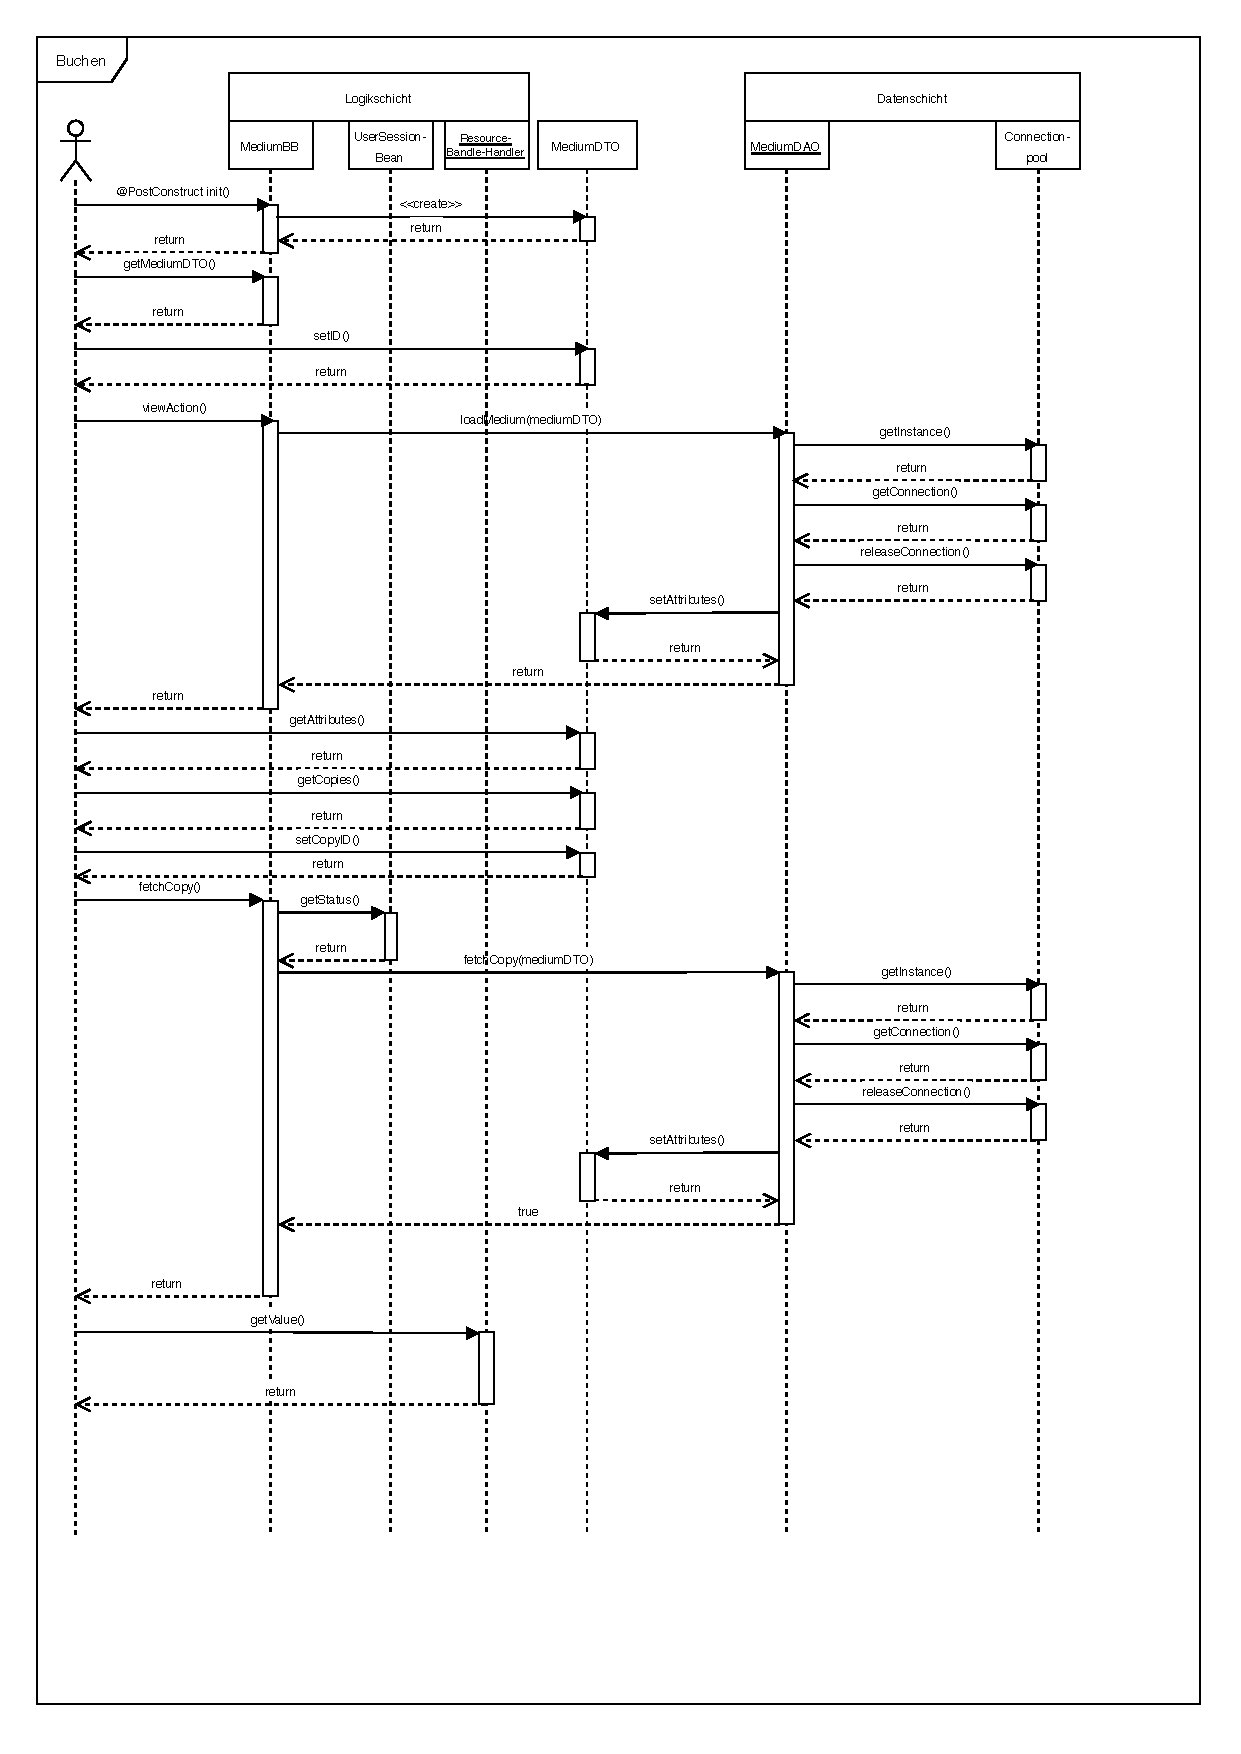
\includegraphics[width = 50em]{Sequenzdiagramm-success-v2}
    \caption{Interaktionen beim erfolgreichen Buchen eines Medium-Exemplares}
    \label{Sequenzdiagramm}
\end{figure}

\restoregeometry
\newpage

\newgeometry{left=0cm,right=0cm,top=0cm,bottom=2cm}

\begin{figure}[h]
    \centering
    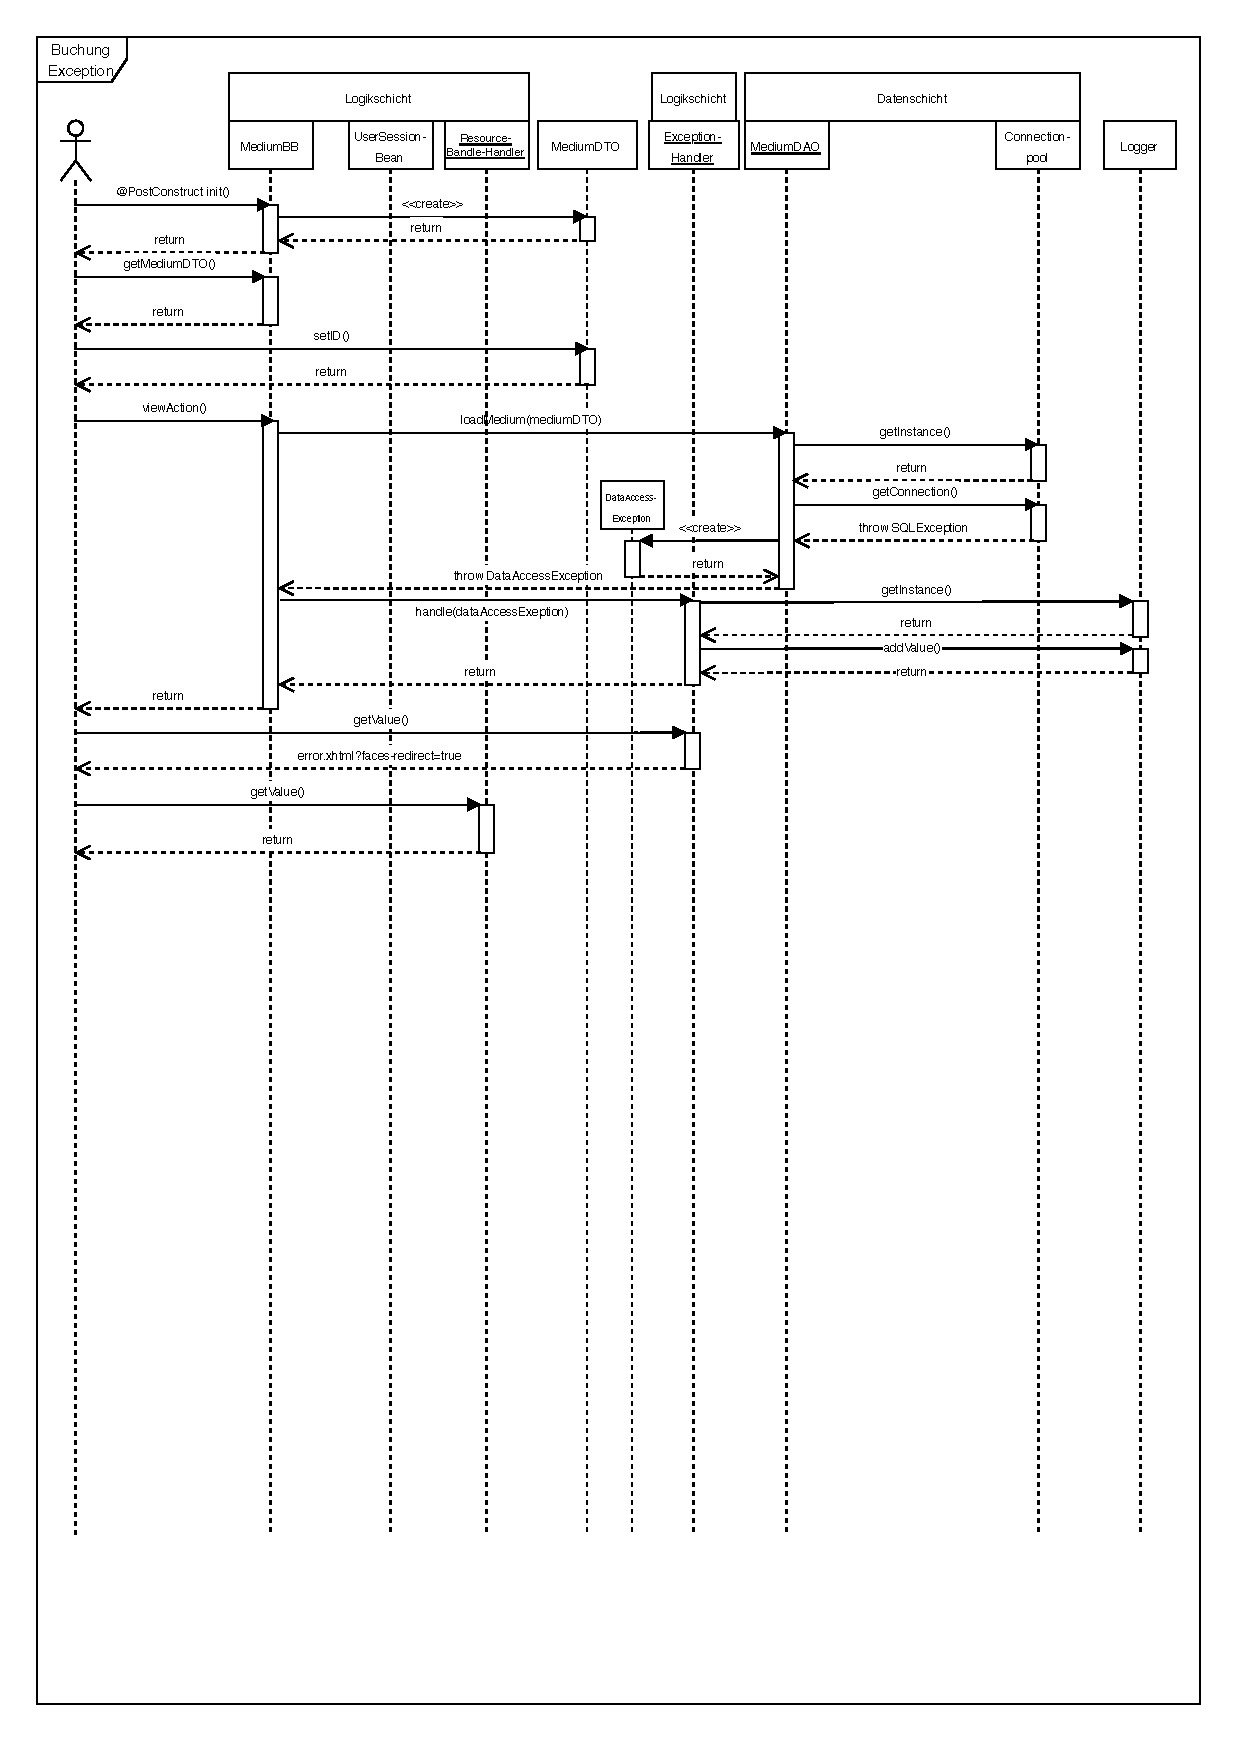
\includegraphics[width = 50em]{Sequenzdiagramm-exception-v3}
    \caption{Interaktionen beim Buchen eines Medium-Exemplares mit fehlender Datenbankverbindung}
    \label{Sequenzdiagramm}
\end{figure}

\restoregeometry
\newpage

%--ER-Modell--------------------------------------------------------------------------------------------------------------------------------------------------------------------------
\section{ER-Modell}
\sectionauthor{Jonas Picker}

\newgeometry{left=0cm,right=0cm,top=0cm,bottom=0cm}

\begin{figure}[h]
    \hypertarget{ERDia}{}
    \centering
    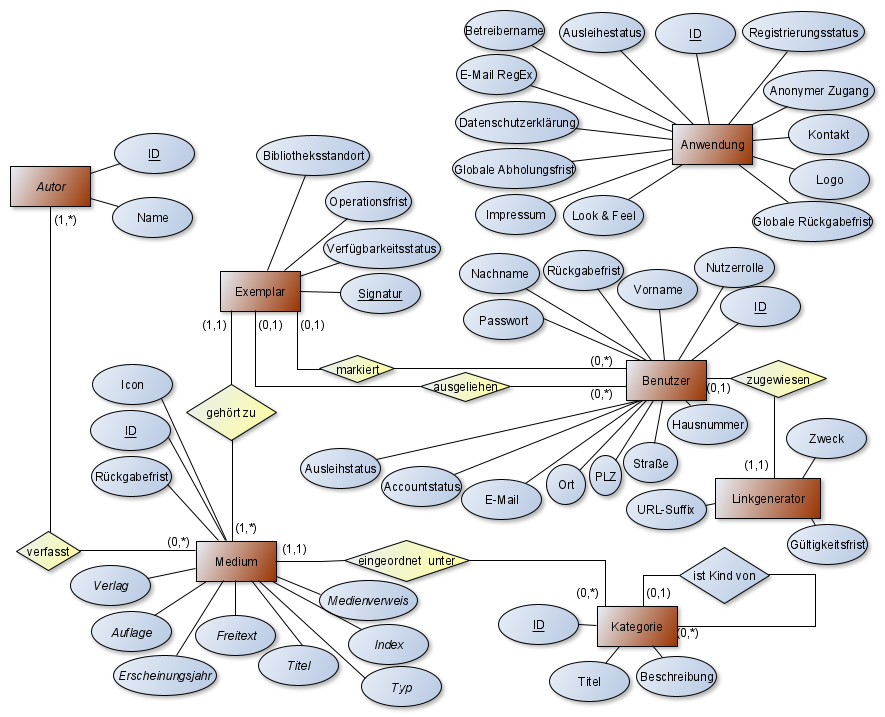
\includegraphics[angle = 270, width = 60em]{ER-Diagramm}
    \caption{Entity-Relationship Diagramm}
    \label{ER-Diagramm}
\end{figure}

\restoregeometry
\newpage

\subsection{Legende}
Beschreibung des \hyperlink{ERDia}{ER-Diagramms}: \\
\\
\textbf{Medium:} Diese Entität modelliert die von der Bibliothek verwalteten Medien. Außer des Primärschlüssels besitzt sie mindestens ein zugehöriges Exemplar und eine variable Anzahl von Attributen. Der \hypertarget{Standartattributsatz}{Standartattributsatz} für Medien wird unten aufgeführt. Es können benutzerdefinierte Attribute hinzugefügt werden (PfHft. /F380/) und jedes der folgenden Attribute ist löschbar (PfHft. /F381/):
\begin{center}
\begin{tabular} { c c c }
Titel & Erscheinungsjahr &  Verlag \\
 Medientyp & Version &  Freitext \\
 Autoren &  Index (ISBN/ISSN) &  Link auf elektronische Version \\
\end{tabular}
\end{center}
\textbf{Attribut:} Diese schwache Entität hält den Namen und Wert eines Medienattributs, ihr ist genau ein Attributtyp zugeordnet.\\
\textbf{Attributtyp:} Vom Attribut abhängige, schwache Entität. Hiermit werden dem Attribut zugehlrige Eigenschaften modelliert. 'Vorschauposition' bestimmt, ob und an welcher Stelle das Attribut in der Medienvorschau (z.B. in der Listenansicht der Suchergebnisse) angezeigt werden soll. 'Multiplizität' entscheidet, ob das zugehörige Attribut mehrfach pro Medium mit unterschiedlichen Werten vorkommen kann oder nicht. 'Persistenz' ist eine Markierung für Attribute, die nicht zum modifizierbaren Attributsatz gehören (z.B. die Rückgabefrist für Medien). 'Datentyp' beschreibt die im Attributwert gespeicherten Daten (z.B. 'String' für Textattribute oder 'Image' um Bilder zu speichern). \\
\textbf{Kategorie:} Die mit dieser Entität verbundenen Relationen ordnen jedem Medium genau eine Kategorie zu und modellieren die Kategoriehierarchie (PfHft. /W440/) durch die Selbstbeziehung. Es wird einen unlöschbaren Top-Knoten in der Hierarchie geben, zu dem alle Medien, die nie in eine Kategorie eingeteilt wurden oder deren Kategorie gelöscht wurde, gehören. Sollten alle Medien in benutzerdefinierten Kategorien stecken, hat der Top-Knoten keine zugeordneten Medien und nimmt somit nicht an der 'eingeordnet unter'-Relation teil.\\
\textbf{Exemplar:} Diese schwache Entität ist vom zugehörigen Medium abhängig. Ein bestimmtes Exemplar kann von genau einem Nutzer zur Abholung markiert oder ausgeliehen werden, diese Aktionen schließen sich gegenseitig aus (PfHft. /F310/) und ändern (genau wie eine Rückgabe) den Verfügbarkeitsstatus und die dazugehörige Operationsfrist dementsprechend. 'Signatur' und 'Bibliotheksstandort' halten bibliothekspezifische Kodierungen. \\
\textbf{Benutzer:} Ob ein Benutzer die Ausleihfunktion benutzen kann, wird durch das Attribut 'Ausleihsperre' modelliert. 'Verifizierungsstatus' zeigt hingegen an, ob der Nutzeraccount bereits den Verifizierungsprozess durchlaufen hat (PfHft. /W70/). Das Passwort wird in gehashter Form abgespeichert. Zur Passwortzurücksetzung und E-Mail-Verifikation wird pro Nutzer ein begrenzt gültiges, einzigartiges 'Token' verwendet, um den entsprechenden Link zu bauen. Die 'Rückgabefrist' für Ausleihen eines Benutzers wird ebenfalls modelliert.\\
\textbf{Registrierter Nutzer:} Diese Nutzer haben positiven 'Verifizierungsstatus'.\\
\textbf{Bibliotheksmitarbeiter:} Diese Entität modelliert die Rolle der Bibliotheksmitarbeiter.\\
\textbf{Administrator:} Diese Entität modelliert die Rolle der Administratoren. Die von der Benutzerentität ausgehende Hierarchie soll die inklusiven Rollen im System modellieren.  \\
\textbf{Adresse:} Vom Benutzer abhängig. Enthält die Bestandteile einer Nutzeradresse als Attribute. \\
\textbf{Anwendung:} Hier werden die setzbaren globalen Variablen und Anwendungseinstellungen modelliert. 'Anonymer Zugang' bestimmt die Berechtigungen anonymer Nutzer beim Besuchen des Webspaces (PfHft. /F10/), während 'Registrierungsstatus' eine offene (in diesem Fall gilt der 'E-Mail RegEx') oder geschlossene Registrierungsfunktion modelliert (PfHft. /F20/). 'Ausleihenstatus' steht für das Umschalten des Systems zur manuellen Freischaltung der Ausleihfunktion. Aus dem 'Mahungsversatz' ergibt sich der Zeitpunkt vor Ablauf einer Rückgabefrist, an dem eine automatische Benachrichtigung versendet wird (PfHft. /F240/). \hypertarget{Farbschemaattribut}{'Farbschema'} merkt sich das zuletzt ausgewählte Farbschema. \\

\end{document}

